%!TEX program = xelatex
\documentclass{scrreprt}
\usepackage{scrhack}
\usepackage{setspace}
\setstretch{1.3}

\voffset=2em

\KOMAoptions
{
  draft,
  fontsize=12pt,
  listof=numbered,
  headlines=4,
  parskip=half,
  BCOR=10mm,
  DIV=10,
}

\usepackage[automark,headsepline]{scrlayer-scrpage}
\ihead{}
\chead{}
\ohead{\headmark}
\ifoot{}
\cfoot[\pagemark]{\pagemark}
\ofoot{}

\usepackage[english]{babel}

\usepackage[datesep=.]{datetime2}
\DTMsetstyle{ddmmyyyy}

\usepackage[autostyle]{csquotes}

\usepackage[backend=biber,style=numeric,urldate=iso8601,date=iso8601]{biblatex}
\addbibresource{Bibliography.bib}

% Alternative to `Helvetica': TeX Gyre Heros
% Alternative to `Bookman Old Style': TeX Gyre Bonum
\usepackage{fontspec}
\setromanfont{TeX Gyre Bonum} % Enhanced version of `Bookman Old Style'.
\setmonofont{Consolas}
% \setsansfont{TeX Gyre Heros} % Replacement for Helvetica.
\setsansfont{Arial} % Replacement for Helvetica.

% Choose default font family.
%
% Options:
%   \rmdefault   Use the serif font family as default.
%   \sfdefault   Use the sans-serif font family as default.
%   \ttdefault   Use the monospace font family as default.
\renewcommand{\familydefault}{\sfdefault}

\usepackage{ifdraft}
\usepackage{amsmath}

\PassOptionsToPackage{draft}{graphicx}
\usepackage{graphicx}

\usepackage{wrapfig}

\usepackage[toc,page]{appendix}

% To disable todonotes: [disable]
\usepackage{todonotes}
\newcommand{\tbd}[0]{\todo[inline, nolist, color=yellow!30]{\centerline{To Be Done}}{}}
\newcommand{\proofread}[0]{\todo[nolist, fancyline, color=cyan!60]{\centerline{Proof-read}}{}}
% Put todo notes on the left side
\reversemarginpar
\setlength{\marginparwidth}{3.2cm}

\usepackage{xcolor}
\definecolor{CodeComment}{gray}{0.4}
\definecolor{CodeKeyword}{rgb}{0.0,0.0,0.8}
\definecolor{CodeString}{rgb}{0.0,0.3,0.0}

\usepackage{listings}
\lstdefinestyle{MyCppInline}
{
  language=[11]C++,
  % commentstyle=\color{CodeComment},
  % keywordstyle=\color{CodeKeyword},
  % numberstyle=\ttfamily\color{CodeComment},
  % stringstyle=\color{CodeString},
  basicstyle=\ttfamily,
  breakatwhitespace=false,
  breaklines=true,
  captionpos=b,
  keepspaces=true,
  numbers=left,
  numbersep=5pt,
  showspaces=false,
  showstringspaces=false,
  showtabs=false,
  tabsize=2
}
\lstdefinestyle{MyCppFloat}
{
  language=[11]C++,
  % commentstyle=\color{CodeComment},
  % keywordstyle=\color{CodeKeyword},
  % numberstyle=\ttfamily\color{CodeComment},
  % stringstyle=\color{CodeString},
  basicstyle=\scriptsize\ttfamily,
  breakatwhitespace=false,
  breaklines=true,
  captionpos=b,
  keepspaces=true,
  numbers=left,
  numbersep=5pt,
  showspaces=false,
  showstringspaces=false,
  showtabs=false,
  tabsize=2,
  frame=single,
  emphstyle={\underbar}
}
\lstdefinestyle{MyXML}
{
  language=XML,
  % commentstyle=\color{CodeComment},
  % keywordstyle=\color{CodeKeyword},
  % numberstyle=\ttfamily\color{CodeComment},
  % stringstyle=\color{CodeString},
  basicstyle=\scriptsize\ttfamily,
  breakatwhitespace=false,
  breaklines=true,
  captionpos=b,
  keepspaces=true,
  numbers=left,
  numbersep=5pt,
  showspaces=false,
  showstringspaces=false,
  showtabs=false,
  tabsize=2,
  frame=single,
  emphstyle={\underbar}
}
\lstset{style=MyCppInline, frameround=tttt}
% \renewcommand\lstlistoflistingsname{List of Listings}

\usepackage{hyperref}
\hypersetup{
  final,
  bookmarksnumbered
  % hidelinks
  % colorlinks,
  % citecolor=black,
  % filecolor=black,
  % linkcolor=black,
  % urlcolor=black
}

\usepackage[all]{nowidow}

% Note: The glossaries package needs to be loaded as late as possible to
%       increase compat with other packages.
\usepackage[acronym,toc]{glossaries}
\loadglsentries{Main/Glossary.tex}
\makenoidxglossaries

% \usepackage[parfill]{parskip}

\usepackage{hhline}

\usepackage{tabu}

\usepackage[nopar]{lipsum}
\setlipsumdefault{1}

\emergencystretch=1em

\hyphenation{LunarG}


\usepackage{ifthen}
\newboolean{hdm}
\setboolean{hdm}{true}

\usepackage[perpage]{footmisc}

\usepackage{comment}

% Set the depth of the numebering scheme for chapters, section, subsection, etc.
\setcounter{secnumdepth}{3}

\begin{document}
  %
  % Title Page
  %

  \ifthenelse{\boolean{hdm}}
  {
    \begin{titlepage}
      \begin{centering}
        \todo[inline, nolist, color=red!64]{\centerline{DRAFT}}{}

        \large

        Masterarbeit im Studiengang \\ \textit{\Large Computer Science and Media}

        \vspace{\fill}

        {\fontsize{2.4em}{0}\selectfont\bfseries
          Prototypical Evaluation \par of Vulkan's Low-Level \par Graphics Pipeline
        }

        \vspace{\fill}

        vorgelegt von \\ \textit{\Large Manuel Maier} \\ Matrikelnummer 28535

        an der \\ \textit{\Large Hochschule der Medien Stuttgart}

        am \\ \textit{\Large \DTMtoday}

        zur Erlangung des akademischen Grades eines \\ \textit{\Large Master of Science (M.Sc.)}

      \end{centering}

      \vspace{\fill}

      \begin{tabu}{ll}
        Erstprüfer:  & \textit{Prof. Dr. Stefan Radicke} \\
        Zweitprüfer: & \textit{Patrick Bader, M.Sc.}
      \end{tabu}

    \end{titlepage}
  }
  {
    \titlehead{\todo[inline, nolist, color=red!64]{\centerline{DRAFT}}{}}
    \subject{Master's Thesis \\ Computer Science and Media \\ Hochschule der Medien Stuttgart}
    \title{Prototypical Evaluation \par of Vulkan's Low-Level \par Graphics Pipeline}
    \author{Manuel Maier}
    \date{\DTMToday}
    \publishers
    {
      Supervisors \\
      \textbf{Prof. Dr. Stefan Radicke}\\
      \textbf{Patrick Bader, M.Sc.}
    }
    \maketitle
  }


  %
  % Blank page for physical notes, name entries, etc.
  %
  \newpage
  % \ifthenelse{\boolean{hdm}}
  % {
  %     \begin{tabu}{ |l|X| }
  %       \multicolumn{2}{c}{Masterarbeit} \\
  %       \multicolumn{2}{c}{Computer Science and Media} \\
  %       \multicolumn{2}{c}{Hochschule der Medien Stuttgart} \\
  %       \hline
  %       Titel               & Prototypical Evaluation of Vulkan's Low-Level Graphics Pipeline \\
  %       \hline
  %       Titel bei Anmeldung & Evaluating the Resource Management Possibilities of the Vulkan Graphics API \\
  %       \hline
  %       Autor               & Manuel Maier \\
  %       \hline
  %       Semester            & Wintersemester 2016 \\
  %       \hline
  %       Abgabedatum         & \DTMToday \\
  %       \hline
  %       Matrikelnummer      & 28535 \\
  %       \hline
  %       Kürzel              & mm198 \\
  %       \hline
  %       E-Mail              & mjmaier@gmx.de \\
  %       \hline
  %     \end{tabu}
  % }
  {
    \null
  }
  \thispagestyle{empty}
  \pagenumbering{gobble}

  %
  % Eidesstattliche Versicherung
  %
  \ifthenelse{\boolean{hdm}}{%!TEX root = ../Main.tex

\chapter*{Eidesstattliche Erklärung}

Hiermit versichere ich, Manuel Maier, ehrenwörtlich, dass ich die vorliegende Masterarbeit mit dem Titel: „Prototypical Evaluation of Vulkan's Low-Level Graphics Pipeline“ selbstständig und ohne fremde Hilfe verfasst und keine anderen als die angegebenen Hilfsmittel benutzt habe.
Die Stellen der Arbeit, die dem Wortlaut oder dem Sinn nach anderen Werken entnommen wurden, sind in jedem Fall unter Angabe der Quelle kenntlich gemacht.
Die Arbeit ist noch nicht veröffentlicht oder in anderer Form als Prüfungsleistung vorgelegt worden.

Ich habe die Bedeutung der ehrenwörtlichen Versicherung und die prüfungsrechtlichen Folgen, gem. § 19 Abs. 2 Master-SPO (4 Semester und berufsbegleitend) der \acrshort{hdm}, einer unrichtigen oder unvollständigen ehrenwörtlichen Versicherung zur Kenntnis genommen

\vspace{\fill}

\begin{tabu} to \linewidth { X[3] X X[3] }
  \hhline{-~-}
  {\footnotesize Ort, Datum} & & {\footnotesize Unterschrift}
\end{tabu}
}{}


  %
  % Abstract and acknoledgements.
  %
  %!TEX root = ../Main.tex

\ifthenelse{\boolean{hdm}}
{
\chapter*{Kurzfassung}
\label{Abstract_de}
  Dies ist die Kurzfassung.
  \todo[inline]{Will be composed once the English version is complete.}


\newpage
}
{}

\chapter*{Abstract}
\label{Abstract}
  In recent years, consumer graphics hardware has changed considerably.
  In the past, the hardware consisted only of fixed-function components that performed the necessary computations in a massively parallel manner to transform three-dimensional data to an image displayed on a screen.
  At the same time, APIs to graphics hardware were developed.
  As hardware design changed over the years, mainly to improve on performance, it has also become more generalized and accessible to other kinds of computational tasks\todo{Add ``than computer graphics''?}.
  Traditional APIs had to adjust to these design changes while maintaining compatibility to previously supported designs at the same time.
  This led to an increase in driver complexity, ultimately impacting performance in a negative way.
  New graphics APIs were designed to match recent hardware more closely, one of which is the Vulkan graphics API.

  In this work\todo{Use ``thesis'' or ``document'' instead of ``work''?}, the Vulkan graphics API is presented in three stages.
  At first, an overview of the API itself is provided.
  Afterwards, general instructions on how to set up an environment for developing Vulkan applications are given.
  And finally, the fundamentals of rendering an image using Vulkan are presented with the aid of simplified, prototypical examples.

  %!TEX root = ../Main.tex

\chapter*{Acknowledgements}
\label{cha:Acknowledgements}

These are my acknowledgements.

\todo[inline]{Make proper sentences below.}

\paragraph{Stefan Radicke}
  supervision.
  Lorem ipsum dolor sit amet, consectetuer adipiscing elit. Aenean commodo ligula eget dolor. Aenean massa. Cum sociis natoque penatibus et.

\paragraph{Patrick Bader}
  supervision.
  Lorem ipsum dolor sit amet, consectetuer adipiscing elit. Aenean commodo ligula eget dolor. Aenean massa. Cum sociis natoque penatibus et.

\paragraph{Hannes Pernpeinter}
  discussion, proof-reading.
  Lorem ipsum dolor sit amet, consectetuer adipiscing elit. Aenean commodo ligula eget dolor. Aenean massa. Cum sociis natoque penatibus et.

\paragraph{Christopher Manthei}
  discussion, proof-reading, experience.
  Lorem ipsum dolor sit amet, consectetuer adipiscing elit. Aenean commodo ligula eget dolor. Aenean massa. Cum sociis natoque penatibus et.

\paragraph{Benjamin Thaut}
  ???.
  Lorem ipsum dolor sit amet, consectetuer adipiscing elit. Aenean commodo ligula eget dolor. Aenean massa. Cum sociis natoque penatibus et.

\paragraph{Maria Floruß}
  rubber-ducking, proof-reading, support, help with illustrator.
  Lorem ipsum dolor sit amet, consectetuer adipiscing elit. Aenean commodo ligula eget dolor. Aenean massa. Cum sociis natoque penatibus et.



  %
  % Table of Contents
  %
  \newpage
  \pagenumbering{roman}
  \tableofcontents
  \newpage


  %
  % List of todos.
  %
  % \listoftodos


  %
  % Chapters
  %
  \pagenumbering{arabic}
  %!TEX root = ../Main.tex

\chapter{Introduction}
\label{cha:Introduction}
  \todo[inline]
  {
    Brief introduction of computer graphics. One of the biggest problems: Performance. Especially with virtual reality.

    Maybe mention the author's (that's me!) bias towards game development.

    Mention target audience requirements.

    Explain shader stages of modern graphics hardware somewhere in this chapter.
  }

  % The field of computer graphics poses many challenges.

  % Data is consumed by a pipeline and transformed by complex algorithms, resulting in another set of data that is used in further processing. This transformation process is usually referred to as ``rendering''. In its most simple form, the output of the rendering process is used to present a graphical representation of the input data to the user, typically via a computer monitor peripheral device.

  % Computer graphics is an area of computer science that has many disciplines. Examples are \glspl{gui}, computer vision, sprite graphics, and \gls{3d} modelling. Most relevant to this paper is \gls{3d} computer graphics. \todo{Mention how Vulkan is not only suited for \gls{3d} graphics?} The most typical use case in \gls{3d} computer graphics is to process data, usually three-dimensional geometric data, in order to produce a 2D image which is then presented to the user with the help of a computer monitor. This processing of data is referred to as \textit{3D rendering} or simply \textit{rendering}.

  % While 3D rendering can be implemented in software, special hardware called a \gls{gpu} can be used instead to achieve better performance. The need for such hardware already indicates one of the greatest challenges in 3D computer graphics: performance. The amount of data involved in 3D rendering can become quite large. As an example, assume the following:

  % \todo{Explain what a Vertex is and how graphics hardware produces faces etc.}

  % The aforementioned three-dimensional geometric data can be given in many different ways. The ideal way of representing specific data depends on the use case and the entire 3D graphics pipeline.

  % For the sake of illustration, let's assume a data set that consists only of 3D vertices. In this example, each vertex only has a position defining the absolute location of the vertex in 3D space. This position value is stored as a vector of three floating point numbers. Typically, such floating point numbers are standard IEEE floating point numbers (as per IEEE 754), taking up 32 bits or 4 bytes of memory. Thus, each vertex takes up $3*4 = 12$ bytes of memory.

  % On desktop systems, applications typically don't access the graphics hardware directly. They instead communicate with a driver that manages hardware access. Communication between an applicatin and the driver is done via an \gls{api}. Figure \ref{fig:AppApiDriverOverview} visualizes this relationship. Ideally, the application does not need to know which specific driver it is communicating with as long as the driver is compliant to the \gls{api} specification. This abstraction decouples the application from the hardware and enables it to run on systems with different hardware configurations without altering the application itself. It also enables hardware vendors to manipulate or even reject operations requested by the application, typically to enforce some user-specified global settings. \todo{Explain what kind of settings? Maybe give an example?}

  \begin{figure}
    \centering
    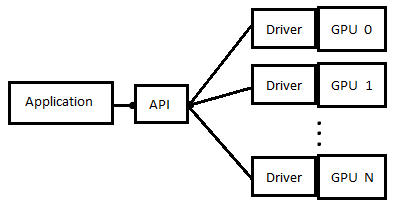
\includegraphics{Main/Images/Application_API_Driver_Overview}
    \caption{Interaction between the application and the hardware via the API.}
    \label{fig:AppApiDriverOverview}
  \end{figure}

  \todo[inline]{Talk about different kinds of graphics \glspl{api} on different systems (D3D, OpenGL on desktop, maybe Metal for OSX, and special \glspl{api} on consoles.)}


  \section{High Level Graphics Workflow}
    \label{sec:GraphicsWorkflow}
    \todo[inline]
    {
      General overview of the stages several resources (vertices, textures, etc.) have to go through.

      Explain the fixed function pipeline.
    }

    \missingfigure{Visualize data flow of data between shader stages.}
    \tbd


  \section{Motivation for a new Graphics API}
    \todo[inline]{Basically write why Vulkan is needed.}

    Graphics hardware is changing rapidly through the years and is highly specialized to do computational work in a massively parallel manner. This makes it not only suitable for graphics computation, but also for general-purpose parallelization of working with large sets of data. These \glspl{api} have grown with the hardware, constantly adapting to it, adding new versions that support different kinds of features and provide different kinds of extensions while maintaining backwards compatability as much as possible. This lead to very complicated \glspl{api} that was getting harder and harder to understand with each new release, especially for beginners.

    \todo[inline]{It might be too obvious that the paragraph above refers to OpenGL. Maybe just make it OpenGL-specific. Would still need to explain why Vulkan is not as abstract as OpenGL. Parts of this is explained below.}

    But not only graphics and compute hardware has changed. The drivers accompanying the hardware also have to stay backwards compatible. They hide and abstract a lot of the low-level functionality that is needed to work properly with the hardware. This abstraction means that the application developer has less control over what is actually done with the data fed to drivers. Since drivers rarely get information about the exact intent of what the developer plans to do with the supplied data, they have to implement heuristics to decide the best course of action.

    This level of abstraction has been criticized by many professional developers over the years, demanding for more low-level control\todo{Reference something here. A paper, in the best case.}. On gaming consoles, low-level control of the hardware was always required, except for Microsoft platforms where the \gls{d3d} technology has always been in use. This meant that console developers were already used to thinking about data flow on a low level and work very closely with the hardware.

    Another aspect is the advent of multi-core CPUs for personal computers in the mid 2000's. Multithreading has become common in CPU programming to achieve better performance. Older graphics \glspl{api}, however, were designed to run on a single thread all the time. Even though these \glspl{api} provide limited support for multithreading by now, they were still originally not designed for it, making it rather difficult to fully utilize multicore performance.

    \todo[inline]{Talk about new \glspl{api} such as D3D12, Mantle, Metal, and also talk about consoles (no specs) that all adress these problems.}


  \section{The Vulkan Graphics and Compute API}
    \todo[inline]{What does it do. Where does it come from. What are people expecting from it. Cross-platform nature (in comparison maybe to PS4's libGNM made specifically for PS4 hardware).}

    \todo[inline]{Insert missing references.}
    The Vulkan \gls{api} was designed by the Khronos Group in collaboration with many industry representatives, including Valve Coroporation, AMD, NVIDIA. Version 1.0 of the Vulkan specification was released on the 16th February in 2016. It was designed to provide low-level control to the developer when interacting with graphics and compute hardware.

    Vulkan was designed with a variety of goals in mind.

    \begin{itemize}
      \item Cross-platform
      \item Keep driver complexity at a minimum
      \item Less driver-side CPU overhead
      \item Enable developers a lot of control over the hardware.
      \item Consistent API
    \end{itemize}

    There are many different kinds of hardware configurations today, ranging from high-end gaming systems to mobile platforms such as smartphones. Vulkan is designed to be used with all of these systems. There will be no special version of Vulkan dedicated to embedded systems as was the case with \gls{gles}.

    As a result of striving for less driver overhead, Vulkan also provides the possibility of reducing CPU and GPU power consumption. The driver implementation will have to make fewer guesses of what the host application is trying to do. It is up to the application developer to tell the Vulkan driver exactly what needs to be done. This way the driver only does as much work as it needs to function properly and less power will be consumed. Hardware vendors will also have an easier time providing robust drivers with less bugs due to reduced complexity.

    Another advantage of Vulkan, being a new API built without worrying about backwards compatability, is the chance of designing a new and consistent API so developers will have an easier time creating applications. For more information about the API structure and common patterns in Vulkan, see chapter \ref{cha:VulkanOverview}.

    Version 1.0 of Vulkan was not entirely built in-house at Khronos Group but is in part based on components of AMD's Mantle API, which was donated to the Khronos Group.


    \subsection{Vulkan Competitors}
      \todo[inline]{OpenGL, Direct3D11, Direct3D12, libGNM (PS4), OpenCL}

      Other \glspl{api} exist that are direct competitors to Vulkan.

      \gls{opengl} is Vulkans predecessor and provides a higher level of abstraction from the hardware. It is a very successful API running on several different platforms with varying hardware configurations. Due to its level of abstraction, \gls{opengl} drivers are very complex and do a significant amount of work on the CPU in order to match abstract commands to the hardware.

      Special flavors of \gls{opengl} exist, such as \gls{gles}, which is a subset of \gls{opengl} to enable hardware-accelerated graphics processing on embedded systems such as smartphones and tablets.

      The \gls{d3d} family of \glspl{api} is developed by Microsoft and only supports Microsoft platforms such as the Windows operating system or the Xbox gaming console. The most recent versions of \gls{d3d} are \acrlong{d3d11} and \acrlong{d3d12}. \acrlong{d3d11} provides a higher level of abstraction from the hardware, not unlike \gls{opengl}. It has been around since the release of Windows 7 in 20??\todo{date}. \acrlong{d3d12}, the latest revision of the \gls{d3d} specification released in 2015\todo{exact date?}, is comparable to Vulkan in terms of of hardware abstraction. It provides much more control to the developer over the hardware.

      \todo[inline]{Mac OS X: Metal}

      \todo[inline]{Gaming console graphics libraries.}

      \todo[inline]{OpenCL as compute API}


  \section{Document Structure}
    \todo[inline]{The structure and content of this document.}

    \tbd

  %!TEX root = ../Main.tex

\chapter{Vulkan API Overview/Workflow}
\label{cha:VulkanOverview}
  \todo[inline]
  {
    The Vulkan Graphics \acrfull{api} workflow, object creation, patterns (vkCreate/vkDestroy, vkAllocate/vkDeallocate), synchronization.

    Listing and short explanation of Vulkan components such as buffers, images, command buffers.

    Note that when talking about a ``device'', a logical device is meant. When referring to the actual hardware component the term ``physical device'' will be used.

    Mention queues and queue families somewhere before the Synchronization section.
  }
  \todo[inline]{Refer to Vulkan spec.}

  This chapter provides an overview of the Vulkan API and explains some concepts in more detail. In some places an abbreviated form is used when referring to several Vulkan commands at once, e.g. \lstinline{vkPlaceholder*} would refer to all Vulkan commands that begin with the character string ``vkPlaceholder'', e.g. \lstinline{vkPlaceholderCommand}. The asterisk is used as a wildcard character.

  Vulkan uses the terms ``host'' and ``device'' to refer to the CPU and GPU, respectively, when describing data flow or memory visibility. These terms will be used in this chapter as well with the same meaning.

  \section{Workflow and Patterns}
  \label{sec:WorkflowAndPatterns}
    The Vulkan API was designed to be consistent and explicit. Many patterns can be found in the Vulkan code style that make it easier for the developer to use the API effectively. This section is a walkthrough of the basic steps that need to be taken to set up a Vulkan graphics pipeline to present an image to a display.

    Vulkan makes use of handle types to allow the developer to track objects created with the API. The first object that has to be created is a Vulkan instance. The Vulkan instance can be used to query available physical devices that provide Vulkan support. These physical devices can be queried for certain capabilities, such as supported image formats and hardware features, to aid in deciding which physical device to use for the application. A physical device can subsequently be used to create a logical device, or just device. The number of devices created from a physical device is not limited. When a device is create, all queues associated with it are created as well. This is why there is no \lstinline{vkCreateQueue} but rather \lstinline{vkGetQueue} command. Among other things, devices are used to allocate Vulkan objects or GPU memory. Changes made on Vulkan objects do not have global side-effect observable with the regular Vulkan API. However, drivers and Vulkan layers or extensions are free to modify their own state across Vulkan object boundaries.\todo{Redundant sentence? This should be a given.}

    \todo[inline]{Describe/mention GPU queues in the introduction chapter.}

    Once a device handle has been acquired the developer can create a swapchain to establish a connection between a specific queue on the device and a platform specific presentation engine. A swapchain contains a number of ``presentation images'' the contents of which are produced by the graphics pipeline. These ``presentation images'' are regular Vulkan image objects in a specific format.

    In order to produce images for the presentation engine to consume via the swapchain, a graphics pipeline needs to be created. This graphics pipeline consists of one or more render pass objects that hold information about how to complete a rendering step. Examples of the render pass state that has to be set is the used pipeline stages, such as vertex or fragment shader stages or compute shader stages, as well as setting framebuffer attachments. Render passes can be organized into subpasses which can be set up to depend on other subpasses, e.g. for post-processing.

    With a graphics pipeline in place, command buffers can be used to record rendering commands such as copying device memory to another location or issueing drawing commands. In order to record command, the command buffer needs to set into recording mode. For more information about command buffers, refer to chapter~\ref{cha:GpuResources}.

    \todo[inline]{Put the following into a subsection?}

    Creating Vulkan objects is done by calls to \lstinline{vkCreate*} commands which take a pointer to \lstinline{Vk*CreateInfo} structures and return a handle to the created object. These info structures contain parameters used by the creation command to create the requested type of Vulkan object. The contents of such info structures are specific to each creation command and require the developer to consult the Vulkan specification in order to provide correct input data. Destroying Vulkan objects is done by passing an object handle to those \lstinline{vkDestroy*} commands that exactly correspond to the \lstinline{vkCreate*} command that created the object in the first place. The commands \lstinline{vkCreateBuffer} and \lstinline{vkDestroyBuffer} are examples for this.

    When Vulkan objects are allocated from memory pools, or directly from device memory, calls to \lstinline{vkAllocate*} commands have to be made. These commands are accompanied by \lstinline{vkFree*} commands that return resources to their origin where they originally were acquired from. The general rule is that all objects allocated from pools are released as soon as the pool itself is released. Using Vulkan objects that are released results in undefined behavior, similar to using deallocated memory in C/C++.

    Unlike other APIs, Vulkan does not do any object tracking or reference counting to manage object life times. It is the responsibility of the developer to destroy or free Vulkan objects at the appropriate times, i.e. when they are no longer in use and will not be used in the future by either the host or the device.

    Vulkan objects are not designed to be thread-safe. This means that accessing or modifying a Vulkan object from more than one thread at once can lead to race conditions or other undesirable behavior. It is the responsibility of the developer to employ proper synchronization mechanisms on the host to ensure Vulkan objects are never accessed concurrently.

  \section{Layers and Extensions}
  \label{sec:LayersAndExtensions}
    \todo[inline]{Layers are instance-only, extensions are both on the isntance-level as well as the device-level.}

    Vulkan is designed to be extensible by thirdparty developers. The two mechanisms provided are called layers and extensions.

    A layer in Vulkan can be thought of as an observer to the API calls done by the developer. It does not add new types or commands the developer can use directly.\todo{Illustration of Vulkan with some layers between it and the user}\todo{Elaborate more to make it crystal clear. Make sure to mention no layers are needed.}

    The LunarG SDK, for example, comes with a set of layers to validate usage of the Vulkan API. This is extremely useful during development as it allows the developer to focus on their code rather than the perfect use of the Vulkan API. It should also be noted that bare Vulkan, without any validation layers enabled, does not do any error checking. When the developer passes an invalid combination of flags to some Vulkan function, it is undefined behavior and has to be corrected by the developer.

    Layers can only be created on the instance-level. Until version x.x.x.x \todo{Find out the exact version.}, the developer was able to create device-level layers, but these are deprecated in Vulkan version x.x.xx.x by now.

    \todo[inline]{Pull out neutral descriptions of layers/extensions and put the examples in their own paragraph.}

    As opposed to layers, extensions are able to provide new or add to existing functionality. The motivation for extensions is to keep the Vulkan core functionality small and provide specific functionality via such extensions. In fact, the Khronos Group itself provides built-in extensions for both common and platform specific functionality. An example of an extension that adds platform independent functionality is the \lstinline{VK_KHR_swapchain} extension. It adds several types and commands to create and interact with a swapchain. The concept of a swapchain itself is independent of the platform but it requires the help of platform specific functionality in order to work. On Windows platforms, for example, the developer needs to enable the \lstinline{VK_KHR_win32_surface} extension in order link a swapchain to a Win32 window. From a developer's perspective, they do not have to care about distinguish between platforms when creating a swapchain but they do have to when creating and connecting the swapchain to a surface.

    Extensions can be enabled on both instance-level and device-level. Instance-level extensions provide functionality that is generally independent of the hardware.

    An example for an instance-level extension is \lstinline{VK_EXT_debug_report}. It enables the developer to provide a callback function that is used by Vulkan layers or extensions to communicate with the developer. If validation layers are enabled, this is how they would tell the developer about any validation concerns or violations. An example for a device-level extension is the aforementioned \lstinline{VK_KHR_swapchain} extension. Not all physical devices have to be capable of rendering graphics images. In the end it is up the extension author on which level they provide their extension.

  \section{Memory Management and Resources}
  \label{sec:MemoryManagement}
    \todo[inline]{
      Allocate memory separately and then binding it to resources. Decoupled on purpose for custom management and reuse.

      Introduce buffers, images, global memory and command buffers.


      Command buffers have their own state. Used with vkCmd commands. Are submitted to a queue. Submissions can be executed out of order.

      Investigate: execute commands out of order within the same submission? If no barrier is present, of course.
    }

    Memory management is an important topic in Vulkan.

    \tbd

  \section{Pipelines and Render Passes}
  \label{sec:RenderPasses}
    \todo[inline]
    {
      Distinction between graphics and compute pipeline.

      Pipeline consists of a render pass that may have sub-passes. Pipeline inheritance.

      Pipeline Cache and optimization by storing it on disk.
    }
    \tbd

  \section{Shader Language: SPIR-V}
    \todo[inline]{\acrfull{spir-v}}

    Shader programs are supplied to Vulkan in \acrfull{spir-v} format. \acrshort{spir-v} is a high-level graphics and parallel compute programming language provided in a binary format. The specification is entirely maintained by the the Khronos Group.

    \todo[inline]{Mention tools for SPIR-V.}

    \todo[inline]{Par below needs expanding. Goal is to describe why SPIR-V is a good thing and how people benefit from it.}
    One might wonder why the Khronos Group chose to only support an intermediate representation for shader programs instead of using something like the \acrfull{glsl} that is already in wide-spread use. \todo{Mention OpenGL supports SPIR-V now as well?}

  \section{Synchronization}
    \todo[inline]{Describe what Vulkan offers and discuss the individual use-cases as well as their performance impact.}

    \todo[inline]{Maybe reduce the use of `Vulkan was designed to' throughout the document?}
    Vulkan was designed to run concurrently. Synchronization is the responsibility of the application (mainly). in order to do so, Vulkan provides four types of synchronization primitives: fences, semaphores, events, and barriers. These synchronization primitives can be used to insert execution and memory dependencies in various circumstances.

    \todo[inline]{Explain execution and memory dependencies here?}

    \subsection{Fences}
    \label{sub:Fences}
      A fence is a synchronization primitive used to determine the execution status of submitted operations executed on a queue. Such a fence can only be in one of two states: not signaled and signaled. The status of a fence is visible to the host. The device itself does not use the status of a fence directly.

      In practice, a fence is most commonly used with the \lstinline{vkQueueSubmit} command, which is used to submit work to a device queue that were previously recorded to command buffers. The application can query the fence for its status using \lstinline{vkFenceGetStatus} which determines whether the fence was signaled or not. Waiting for a fence to be signaled essentially means waiting for all of the submitted work on the queue to be finished.\todo{Make clear it's only the work that was given in the same queue submission as the fence}{} In order to wait for a fence to be signaled in a blocking\todo{Sugarcoat the term `blocking' a bit?}{} fashion the \lstinline{vkWaitForFences} command is used.

    \subsection{Semaphores}
    \label{sub:Semaphores}
      A semaphore is similar to a fence, as discussed above in \ref{sub:Fences}\todo{Should I omit this?}, except that its status is only visible to the device. It can be used to synchronize operations within the same and between different device queues.

      The most common use case for Vulkan semaphores in a graphics application is when presenting swapchain images to the presentation engine. First, the commands to create the final image have to be recorded to a command buffer. This command buffer then needs to be submitted to a queue in order to be executed. When submitting to the queue, a semaphore can be provided that will be signaled once the queue has finished executing all submitted commands. The same semaphore can be used when issuing the swapchain presentation command. When everything is set up like this, the presentation engine will effectively wait for the commands to produce the final image and then present it as fast as possible.

      Note that a fence can be used to achieve the same results except that it would require the host to actively wait for the queue to finish executing, stalling any other CPU operations that could have been executed in that time. Using the semaphore in this case will result in better performance.

    \subsection{Events}
    \label{sub:Events}
      Events are used to synchronize from host to device or from device to device in a bidirectional manner. Like semaphores and fences, events are in either a signaled or in a not-signaled state. Events are inserted into command buffers in order to allow the device to signal them. This allows for more fine-grained synchronization between commands and to signal command completion the host. Unlike a fence, an event can be inserted at any point in the command buffer stream and thus can be used to query for synchronization without requiring that all commands in the submitted command buffer have completed execution.

      The way events work could be taken advantage of in a batch resource transformation scenario. Imagine there are an arbitrary number of images in an application that need to be transformed in some way that is expensive to compute. These transformations could be issued into a single command buffer, inserting a completion event between transformation commands. After submitting this command buffer to the queue, the application can periodically query for completion of the individual transformation commands without the need to wait for the entire submission to finish by using fences or semaphores.

      It must be noted that events are only allowed to be insterted into command buffers that are all submitted to the same queue. This makes them unuseful if cross-queue synchronization is requried.

    \subsection{Barriers}
    \label{sub:Barriers}
      Barriers are used exclusively with commands recorded to command buffers. There are two kinds of barriers in Vulkan. The first kind is called an execution barrier which are used to create explicit dependencies on the completion of specific commands. The second kind is called a memory barrier which are used to depend on memory to be present in a specific form. Both kinds of barriers are combined in Vulkan as a pipeline barrier.\todo{Add illustration of floating commands above and below a pipeline barrier.}

      \begin{figure}
      \caption{Illustration of a pipeline barrier insterted between commands in a command buffer.}
      \centering
      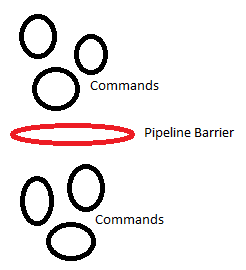
\includegraphics{Main/Images/PipelineBarrier}
      \label{fig:PipelineBarrier}
      \end{figure}

      By inserting a memory dependency, the application indicates to the API that all memory operations need to be finished on a specified resource or memory region once the inserted barrier has been reached. Otherwise all following commands are not able to begin executing. Analogously, an execution dependency requires all previous commands to have finished execution before starting to execute other commands inserted after the barrier.

      There are three types of memory barriers in Vulkan: Global memory barriers, buffer memory barriers, and image memory barriers.

      \subsubsection{Global Memory Barriers}
        \todo[inline]
        {
          Investigate: Are these truly global memory barriers? The spec reads ``applies to memory accesses involving all memory objects that exist at the time of its execution'' which seems very heavyweight.
        }
        Global memory barriers introduce a dependency to all memory objects that exist at the time of execution of the barrier. All prior memory access operations, whether they are read or write operations, must have finished before the barrier finishes execution.

        Such heavy-weight memory dependencies are not needed if the memory in use is entirely cache coherent. In other words, if the rest of the system ensures that all caches are flushed at appropriate times, memory accesses from other parts of the system will be consistent and up-to-date\todo{Double-Triple-Check whether this is actually correct.}.

      \subsubsection{Buffer Memory Barriers}
        Buffer memory barriers introduce a memory access dependency on a specific region of memory associated with a buffer object. That region may encompass the entire buffer and is specified in terms of an offset, relative to the beginning of the buffer, and a size value.

        This kind of barrier can be used to transfer ownership of a buffer region to another queue family or to change access flags of that region. Transferring ownership of that buffer region to another queue family is only possible if this kind of operation has been enabled for that buffer at the time it was created. Access flags are used to control how the buffer region is accessed. They could be used to make the memory region read-only, for example, or enable host access for it.

      \subsubsection{Image Memory Barriers}
        Image memory barriers are similar to buffer memory barriers. They can be used to transfer ownership image regions to another queue family, modify access flags, and to change the image layout. An image region is specified differently from a buffer region of the fact that images need not be stored linearly in device memory\todo{Refer to wherever image tiling is explained}.

        Transferring ownership of an image region is only possible if the image was set up correctly at creation time. Modifying access flags has the same effect as with modifying access flags on a buffer region.

        Changing the layout of the image is an important operation on Vulkan images. For example, it is required for swapchain images in order to be presentable. The presentation engine requires swapchain images to be in a specific layout when presenting them so the application must ensure that the image has that specific layout before attempting to issue the presentation command. Since the presentation layout is only meant for use by the presentation engine, the application has to use another image memory barrier to change the layout into something that can be used by the host application.

    % Fences are

    % There are semaphores, fences, and pipeline barriers.

    % Fences are used to ... and can be waited on using the function \lstinline{vkWaitFences}. Fences are like

    % \todo[inline]{Illustrate a pipeline barrier?}
    % As mentioned in section \ref{sec:CommandBuffers}, commands recorded in a command buffer can be executed out-of-order\todo{Is this \textbf{really} true?} on the queue it is submitted on. The developer can explicitly synchronize
    % Pipeline barriers are used to synchronize execution state and
    % Pipeline barriers are used to ensure all memory operations have finished at a certain point in the pipeline. These barriers are inserted into a command buffer using the \lstinline{vkCmdPipelineBarrier} command. A  common use-case is transitioning a Vulkan image from one layout to another, e.g. from a layout optimized for presentation purposes to a layout optimized for

  \section{Interaction with the Operating System}
    \todo[inline]
    {
      Windowing system, specific Vulkan extensions per OS.

      \textbf{Kill this section?}
    }

  %!TEX root = ../Main.tex

\chapter{Vulkan Development Environment}
\label{cha:EnvSetup}
  % \todo[inline]{Proper introduction to the chapter}

  % This chapter is a guide to setting up a Vulkan development environment in the context of \gls{ccpp} on a \gls{windows} operating system.

  % As can be expected, the steps required to setup a Vulkan environment depend on the development platform of choice.

  This chapter describes some practical aspects of Vulkan development and acts as a guide in setting up a Vulkan development environment.
  As can be expected, the steps required for such a setup depend on the kind of platform to be developed on.
  This chapter introduces the Vulkan Common Loader, which is used to interface with \glspl{icd} and Vulkan layers, the LunarG Vulkan \gls{sdk}, how to develop shaders for Vulkan applications, and discusses debugging and profiling capabilities.

  \section{Hardware Vendor Support}
  \label{sec:HardwareVendorSupport}
    Using and developing Vulkan applications requires support from the hardware.
    Information about Vulkan support for a particular piece of hardware can usually be found in the manual or on the hardware vendor website.
    There are also third-party resources that can be consulted to check whether a particular piece of hardware provides Vulkan support.
    The \textit{Vulkan Hardware Database}~\cite{vulkangpuinfo} is one such resource.
    This database even provides an overview of the supported hardware features and device extensions.

    In order to support Vulkan, hardware vendors have to provide driver implementations for the platform the user is targeting.
    These driver implementations are called \acrfullpl{icd}.
    How an \gls{icd} is chosen by the application is described in section~\ref{sec:VulkanLoader}.

    At the time of writing, \gls{amd}, \gls{nvidia}, as well as \gls{intel} are known to provide Vulkan-enabled hardware and drivers for several operating systems~\cite{practicalvkgdc16}.
    In the early days of Vulkan, \gls{amd} and \gls{nvidia} only provided beta-quality \glspl{driver} but have released consumer-grade versions by now.
    \gls{intel}, on the other hand, only provides beta-quality \glspl{driver} for Windows operating systems and does not intend to release consumer-grade \glspl{driver} on that platform for the time being~\cite{intelvulkandriversonwindows}, although drivers for Linux are available.

  \section{Vulkan Header}
  \label{sec:VulkanHeader}
    The Vulkan header file is generated from a more abstract representation called the Vulkan API Registry.
    The most recent version can be found in the Vulkan-Docs repository on \gls{github}, which can be found in the Khronos Vulkan Registry~\cite{vulkanregistry}.
    This repository contains the generated \gls{ccpp} header file.
    It also contains the file \lstinline{vk.xml} and a set of tools to generate the Vulkan header from it.

    \lstinputlisting[
      label=lst:VkFenceCreateInfo_vkxml,
      caption={The definition of \lstinline{VkFenceCreateInfo} as found in \lstinline{vk.xml}.},
      style=MyXML,
      float
    ]
    {Main/Listings/VkFenceCreateInfo_vkxml.xml}
    \lstinputlisting[
      label=lst:VkFenceCreateInfo,
      caption={The result of generating C bindings from listing~\ref{lst:VkFenceCreateInfo_vkxml}.},
      style=MyCppFloat,
      float
    ]
    {Main/Listings/VkFenceCreateInfo.txt}

    The \lstinline{vk.xml} essentially contains annotated C code with XML markup.
    The annotations also contain contextual information, something pure C code could not easily or conveniently provide in a standard way.
    Listing~\ref{lst:VkFenceCreateInfo_vkxml} shows the definition of a Vulkan structure as defined in the \lstinline{vk.xml} file.
    For this particular entry, the resulting Vulkan header file will contain the definition shown in listing~\ref{lst:VkFenceCreateInfo}.

    This additional layer of abstraction is useful to generate the Vulkan API in different ways.
    For example, when using \gls{cpp}, structures and functions may be reorganized into classes and methods instead, resulting in a code style that is more common in \gls{cpp}.
    It also makes it easier to generate native bindings for other programming languages, such as \gls{csharp} or \gls{python}.
    Line~10 of listing~\ref{lst:VkFenceCreateInfo_vkxml} shows the xml attribute \lstinline{optional="true"}.
    It basically states that it is allowed to pass a flags value of zero, i.e. no flags are set.
    Such an annotation would not be possible in regular C code.
    This is the main advantage of expressing the Vulkan API in this abstract format.


  \section{Vulkan Common Loader}
  \label{sec:VulkanLoader}
    The \gls{vkloader} is the interface between Vulkan applications and \glspl{icd}.
    It is an open source project mainly developed and maintained by the Khronos Group.
    It can be found in the Khronos Vulkan Registry~\cite{vulkanregistry}.
    It is written in \gls{c} and can be used by application developers either as a statically or dynamically linked library.
    It ensures that multiple \glspl{icd} can be installed on the same system without interfering with each other.
    It is also responsible for managing optional modules, called \textit{layers} which have been introduced in chapter~\ref{cha:VulkanOverview}.
    These layers are implemented as software libraries.
    There are explicit and implicit layers.
    Explicit layers can only be enabled when the Vulkan application requests these layers explicitly.
    \todo{Elaborate on controlling layer activation}
    This is done when creating a Vulkan instance or a Vulkan device.
    Implicit layers, on the other hand, are activated by default.

    \subsection{Interaction with an ICD}
      As explained in section~\ref{sec:WorkflowAndPatterns}, the first Vulkan object that has to be created by every application is the Vulkan instance.
      This instance can be used to query all layers that are available for that Vulkan instance.
      In this section, the process of loading Vulkan commands and interacting with the \gls{driver} and all layers in-between is looked at in more detail.

      In addition to what has been described so far, a layer is also able to provide several Vulkan \textit{extensions}.
      These extensions may define additional Vulkan commands that can be queried via the \gls{vkloader} using \lstinline{vkGetInstanceProcAddr} and \lstinline{vkGetDeviceProcAddr}, which are Vulkan commands to retrieve addresses of functions that are identified by their name.
      Usage of these Vulkan commands, in the context of a \gls{windows} operating system platform, is demonstrated in listing \ref{lst:VulkanFunctionLoading} as pseudocode.
      % Pseudocode of how these Vulkan commands are used is demonstrated in listing \ref{lst:VulkanFunctionLoading} in the context of a \gls{windows} operating system platform.

      \lstinputlisting[
        label=lst:VulkanFunctionLoading,
        caption={Pseudocode for loading different Vulkan functions using the \gls{vkloader} module on a Win32 platform.},
        style=MyCppFloat,
        float,
        emph={vkGetInstanceProcAddr, vkGetDeviceProcAddr}
      ]
      {Main/Listings/VulkanFunctionLoading.txt}

      On the first line, the \glsdisp{windows}{Windows}~\gls{api} is used to load the \gls{vkloader}, simply called \lstinline{Loader} in the sample.
      On this platform, the \gls{vkloader} for Vulkan specification 1.0 and above is a \gls{dll} and is called \textit{vulkan-1.dll}.

      % Continuing in the sample, the next step is to acquire the function \lstinline{vkGetInstanceProcAddr} from the Loader module.
      Continuing in the sample, the function \lstinline{vkGetInstanceProcAddr} is acquired next from the Loader module.
      The \lstinline{vkGetInstanceProcAddr} function is used to load function addresses from the Loader module that are tied to a specific Vulkan instance.
      This Vulkan instance is passed to the \lstinline{vkGetInstanceProcAddr} function as the first argument.
      The second argument is the name of the function to load.

      On line 3 in the sample, \lstinline{NULL} is passed as the Vulkan instance.
      This is only allowed for a small set of functions that are not directly tied to a specific Vulkan instance.
      \lstinline{vkCreateInstance} is one such function, which is subsequently used to create a Vulkan instance on line 4.
      The first argument to \lstinline{vkCreateInstance} is an instance of the \lstinline{VkInstanceCreateInfo} structure.
      Among other things, this structure is used to enable a set of layers and extensions.
      The underlined elements in listing~\ref{lst:VkInstanceCreateInfo} show the relevant fields in order to enable the respective layers and extensions.

      \lstinputlisting[
        label=lst:VkInstanceCreateInfo,
        caption={Definition of the \lstinline{VkInstanceCreateInfo} structure.},
        style=MyCppFloat,
        float,
        emph={ppEnabledLayerNames, ppEnabledExtensionNames}
      ]
      {Main/Listings/VkInstanceCreateInfo.txt}

      On line~5 of listing~\ref{lst:VulkanFunctionLoading} the address of the Vulkan command \lstinline{vkCreateDevice} is acquired.
      Instead of passing \lstinline{NULL}, this time the actual Vulkan instance is passed.
      This is done in order for the loader to know which active layers have to be notified about this call since they might have registered hooks to intercept the calls when creating a Vulkan device.

      In the next line, a Vulkan device is created using the previously fetched Vulkan command.
      During this call, all active and relevant layers, meaning all those layers that registered a hook for this case, are traversed and notified about this call.
      Similar to the process of creating a Vulkan instance, when creating a device, the application can request certain \textit{device extensions} to be activated.
      As can be seen in listing~\ref{lst:VkDeviceCreateInfo}, the process of requesting these extensions is very similar to requesting instance-level extensions.

      \lstinputlisting[
        label=lst:VkDeviceCreateInfo,
        caption={Definition of the \lstinline{VkDeviceCreateInfo} structure.},
        style=MyCppFloat,
        float,
        emph={ppEnabledExtensionNames}
      ]
      {Main/Listings/VkDeviceCreateInfo.txt}

      \begin{figure}
        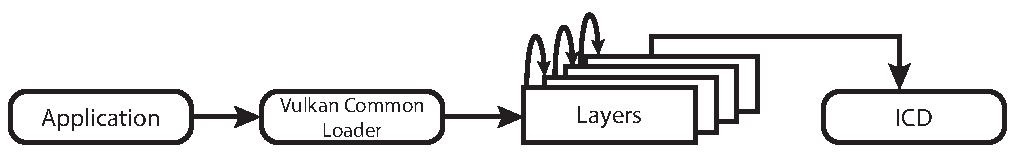
\includegraphics[width=1.0\textwidth]{Main/Images/VulkanLoaderDeviceLayers}
        \centering
        \caption{Communication between the application and an \acrfull{icd} via the \gls{vkloader} when using device-level API calls.}
        \label{fig:VulkanLoaderWithDeviceLayers}
      \end{figure}

      Line~7 of listing~\ref{lst:VulkanFunctionLoading} shows acquiring the address to the Vulkan command called \lstinline{vkGetDeviceProcAddr} which is used to acquire function addresses from a specific \gls{icd}.
      This way, the Vulkan application can get the implementation of a command directly from the \gls{icd}.
      This alleviates the work required from the \gls{vkloader} as it does no longer have to look up the correct \gls{icd} for the context of the current call.

      Lines~8~and~9 are just examples of how a device-specific command is queried and executed.
      Just like before, the \gls{vkloader} will make sure all relevant layers are notified about this call, even though this time it is a device-specific call as opposed to an instance-specific call.

      \begin{figure}
        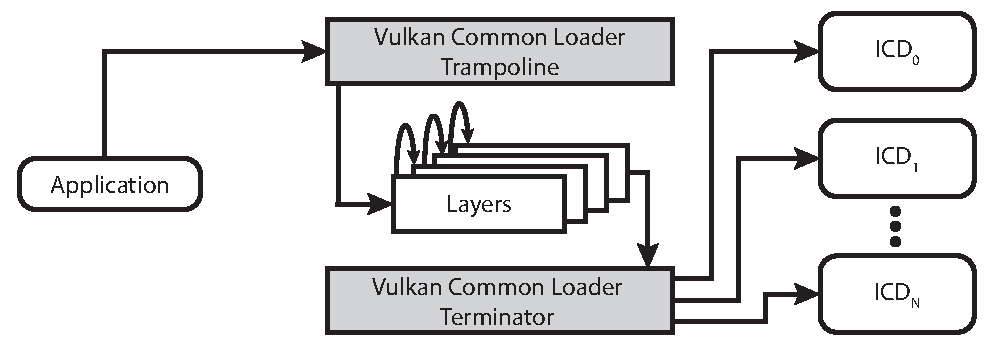
\includegraphics[width=1.0\textwidth]{Main/Images/VulkanLoaderInstanceLayers}
        \centering
        \caption{Communication between the application and the \acrfullpl{icd} via the \gls{vkloader} when using instance-level API calls.}
        \label{fig:VulkanLoaderWithInstanceLayers}
      \end{figure}

      In performance-critical applications care must be taken when activating layers in a production scenario.
      Because every layer is called in order, every layer introduces additional overhead per \gls{api} call.
      See figure~\ref{fig:VulkanLoaderWithInstanceLayers} and figure~\ref{fig:VulkanLoaderWithDeviceLayers} for an illustration of how Vulkan~\gls{api} calls are handled by the \gls{vkloader}.
      Validation layers, for example, are typically not desired in a production scenario.
      At the time of writing there is no standard way to get \gls{icd} modules using the \gls{vkloader}.
      However, because of the \gls{vkloader} being open-source software, a developer is able to extract the relevant loader logic, customizing it to their specific needs.
      This should only be done if absolutely necessary because it requires the developer to maintain their port of the \gls{vkloader} in case future revisions of the original \gls{vkloader} change internal behavior or layer and extension conventions crucial for proper execution of the application.
      Otherwise the developer risks that their application stops working because of incompatibilities.
      After all, internals or conventions introduced by the original \gls{vkloader} are not specified by Vulkan.

      % \todo[inline]{Device extensions are for vendor-specific extensions, such as NV\_glsl that support loading glsl shader code. For more on shaders see sec:EnvShaders.}

      \todo[inline]
      {
        Layers are discovered by the loader via the registry on Windows and in special directories on Unix based platforms.
        Files discovered there are always in JSON format and provide information about the library location and more.
        \lstinline{HKEY_LOCAL_MACHINE\\SOFTWARE\\Khronos\\Vulkan}
      }

      \todo[inline]{Dissect an example JSON file and explain the parts here?}

      \todo[inline]{Mention that the order in which layers are activated matters?}


  \section{LunarG Vulkan SDK}
  \label{sec:LunarGSDK}
    The LunarG Vulkan \gls{sdk}~\cite{lunargvulkansdk} is a \acrlong{sdk} developed by LunarG.
    LunarG is a software company that develops tools and infrastructure for Vulkan development.
    The company itself is sponsored by Valve Corporation.
    The first version of the LunarG \gls{sdk} was released at the same time as version 1.0 of the Vulkan specification.

    Developing a Vulkan application does not require the LunarG \gls{sdk} to be installed.
    For that, only the Vulkan header and \gls{vkloader} are required.
    However, the LunarG \gls{sdk} includes these two components and a number of additional components.
    These components are meant to help making it easier to develop Vulkan applications.
    Aside from the Vulkan header and the \gls{vkloader}, the \gls{sdk} also includes several Vulkan layers, debugging tools, tools that aid in creating shader modules compatible with Vulkan, the Vulkan API documentation, and a range of Vulkan samples and demos as well as a sample-driven tutorial.

    \todo[inline]{Mention the \lstinline{vulkaninfo} command?}


  \section{Shaders}
  \label{sec:EnvShaders}
    As mentioned in section~\ref{sec:Pipelines}, Vulkan expects shaders to be in \gls{spirv} format.
    \gls{spirv} is a binary format and is not meant to be human-readable.
    Instead of writing shaders directly in \gls{spirv} format, they are usually written in \gls{glsl} and converted to \gls{spirv} in a subsequent step.
    The most commonly used tool for this purpose is called \textit{glslangValidator}~\cite{glslangrepo} and is a command-line based tool that is able to validate \gls{glsl} code and to convert it into other representations, specifically \gls{spirv}.
    \todo{Describe what exactly is required. layout=N, binding=N, set=N, \#extension, ...}
    It requires the \gls{glsl} source code to be written in a specific way in order to be converted to \gls{spirv}.

    % \todo[inline]{explain that shaders can be converted in different shader stages, e.g. vertex-, fragment-stage, hence the file endings and filenames}

    \lstinputlisting[
      label=lst:glslangcmd,
      caption={Sample usage of the program called \lstinline{glslangValidator}.},
      style=MyCppFloat,
      float
    ]
    {Main/Listings/glslangValidator.txt}

    Listing \ref{lst:glslangcmd} shows how to convert two shader programs, provided in \gls{glsl} format, to \gls{spirv} using Glslang.
    The \lstinline{-V} switch tells Glslang to convert to Vulkan-compatible \gls{spirv} format.
    The \lstinline{-o} switch is used to control how the output file is named.
    In the first line, the input is the file called \lstinline{Shader.vert} and the output is a file called \lstinline{Vertex.spv}, which will be in \gls{spirv} format.
    The second line does the same transformation for the input file \lstinline{Shader.frag} and the output file \lstinline{Fragment.spv}.

    Another approach is to use a custom-made front-end that would be convertible to \gls{spirv}.
    This might be the favorable approach for many graphics or game engines since these technologies \todo{Do I need references here?}usually have their own abstract representation of shader functionality.
    Being able to directly translate to \gls{spirv} removes the need to translate into some human-readable form first, such as \gls{glsl}, as was the case with \gls{opengl}.


  \section{Debugging and Profiling}
  \label{sec:DebuggingAndProfiling}
    The layered architecture of Vulkan makes it straight-forward for tool developers to provide debugging and profiling capabilities that integrate seamlessly with existing Vulkan applications.
    These tools usually just offer one or more layers, and possibly some extensions, that are either implicitly or explicitly activated.

    The LunarG Vulkan \gls{sdk} comes with a variety of layers, many of which are debugging layers.
    It also provides a layer which combines all debugging layers in one layer in an optimal order called \lstinline{standard_validation}\footnote{Full name: \lstinline{VK_LAYER_LUNARG_standard_validation}}.
    All these debugging layers, including the standard validation layer, are explicit layers that have to be activated when creating a Vulkan instance.
    Layers have been described in section~\ref{sec:LayersAndExtensions} and the careful reader might have noticed that layers do not get back in touch with the Vulkan application directly.
    % \todo{Find out where this extension is coming from? i.e. from which layer. Seems like all layers provide it?!}
    For this purpose the \lstinline{VK_EXT_debug_report} extension is used.
    This extension provides additional Vulkan commands that can be used to supply a callback that will be triggered whenever a layer, that supports the debugging interface, needs to communicate back to the Vulkan application.
    For example, when a validation layer detects erroneous input, it will invoke the supplied debug callback and inform the application of invalid behavior.

    Another tool for debugging, that is also supplied with the LunarG Vulkan \gls{sdk}, is RenderDoc~\cite{renderdoc}.
    RenderDoc is a graphics debugging tool that allows the developer to inspect pipeline states at each \gls{api} invocation.
    RenderDoc has provided \gls{d3d} and \gls{opengl} support for quite some time already but also provides Vulkan support since the release of Vulkan 1.0.
    When RenderDoc is installed, it also installs the implicit layer called \lstinline{VK_LAYER_RENDERDOC_Capture}.
    This means that any Vulkan-enabled application can be debugged using RenderDoc.
    This layer is used to capture \gls{api} calls and track state in that way.
    In order for RenderDoc to work, it has to be hooked up with the Vulkan application that is to be inspected.
    Once hooked up, RenderDoc is rendering a small amount of statistics, such as current frame rate, in the upper left corner of the applications window.
    It also shows which button to press to instruct RenderDoc to capture a frame.
    Once a frame was captured it can be inspected inside of the RenderDoc UI.
    This captured frame contains, among other things, the state of the frame buffers but also records \gls{api} calls, shows their \gls{cpu} execution time, shows bound textures for active shaders, and more.

    Once a Vulkan application is running correctly, the developer might also be interested in whether it runs \textit{efficiently}.
    This is especially important for many real-time applications such as video games.
    Due to the young age of Vulkan, there are not many profiling tools specifically tailored towards Vulkan applications.
    There are some tools that can aid in this regard, though.
    The LunarG SDK, as described in section~\ref{sec:LunarGSDK}, offers API tracing and playback tools.
    These tools effectively record which commands are performed by an application, measuring the execution time of individual commands.
    This can help in tracking down bottlenecks observed on the host-side.
    The RenderDoc Graphics Debugging Tool~\cite{renderdoc} also has the capability of tracking API calls.
    However, tools of this kind are not capable of capturing how the GPU behaves for a given Vulkan application.
    At the time of writing, no Vulkan-specific GPU profiling tool is available as known to the author.

    % For measuring \gls{gpu} behavior on a more general scale, other tools can be used.
    % One such tool is \gls{nvidia} FCAT~\cite{nvidiafcat}.
    % This tool requires a special piece of hardware, called a \textit{capture card}, that captures the output of a graphics card and displays analysis results directly on the attached computer display.
    % Thus, it does not rely on application-specific, internal measurements.
    % Usage of this tool is not wide-spread but
    % Usage of this tool is note wide-spread, but at least some computer magazines use it for benchmarking when comparing different models of graphics and compute harcware~\cite{eurogamer2016:doomvulkan}\todo{citations! At least 2.}.

    The Vulkan \gls{api} itself also provides so-called \textit{timestamp queries}.
    These queries can be used to insert special query commands into a command buffer to write a timestamp value into a \textit{query pool}.
    The results recorded in the query pool can then be read from the host at certain times.
    This enables application developers to implement their own internal \acrshort{gpu} profiling system by taking time samples at application-defined points within command buffers.
    See section~16.5 of the Vulkan specification~\cite{vkspec} for details.

    % \todo{Better phrasing? Make it more formal.}Vulkan has only been around for a short while now.
    \todo{Omit this paragraph?}
    Vulkan is still relatively new technology.
    Existing tools for other graphics \glspl{api} will most likely be extended to also support Vulkan.
    It is also possible that new tools dedicated to Vulkan may be developed by hardware vendors.

  %!TEX root = ../Main.tex

\chapter{Vulkan Rendering}
\label{cha:RenderPipeline}
  \todo[inline, color=red!60]{Rename chapter? Current name matches with the names of the previous chapters.}
  \todo[inline]
  {
    Possible titles:
    Rendering Workflow,
    Applying the Rendering Pipeline,
    Rendering in Vulkan,
    Rendering Commands and Resource Handling/Management,
    Rendering Walkthrough/Guide,
    Specific/Concrete Example of a Rendering Pipeline
  }

  \todo[inline]{Image tiling and layout?}
  \todo[inline]{Resource transformations?}

  This chapter provides an overview of the steps required to render an image using the Vulkan graphics \gls{api}.
  Because there are many ways to perform rendering with Vulkan, a framework is defined that constrains the actual work that needs to be done to a comprehensible amount.

  First, the aforementioned framework is defined.
  Subsequently, the necessary Vulkan \gls{api} calls are show and explained in order to prepare for rendering.
  Following these preparations, recording of the actual rendering commands is shown.
  And finally, in the render loop.
  Section~\ref{sec:MultithreadedRendering} at the end of this chapter provides additional information about multi-threaded rendering in Vulkan.

  Throughout this chapter, listings are presented that show the usage of select Vulkan commands and data structures that are required for rendering.
  It must be noted, however, that these listings are simplified in order to improve legibility.
  Tasks that need to be performed, such as memory allocation, may be shown in an abridged form.

  \section{Framework}
  \label{sec:Framework}
    \todo{Make sure to explain that the image is created only in a single step.}A simple forward renderer is assumed which means that rendering is performed to an image that is presented as soon as possible.
    A camera is used to observe the scene.
    This camera is not fixed, i.e. it may change position or rotation over time.
    The rendered scene will contain a fixed number of objects.
    Each object has fixed geometry and is assigned a position in an application-defined coordinate space.
    The shaders used to render each object is kept very simple.
    Objects do not have textures or other color information and are rendered in a solid color.
    Lighting is restricted to only produce flat shaded surfaces.
    The actual layout of these shaders is shown in section~\ref{subsec:GraphicsPipelineSetup}.

  \begin{figure}
    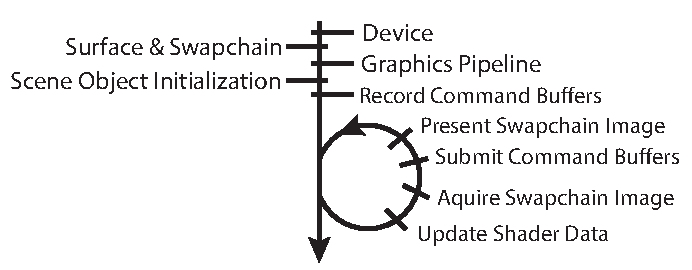
\includegraphics{Main/Images/RenderSetupAndLoopSimple}
    \centering
    \caption{Overview of the setup and execution of a simple forward-renderer in Vulkan as implemented in chapter~\ref{cha:RenderPipeline}.}
    \label{fig:RenderSetupAndLoopSimple}
  \end{figure}

  Figure~\ref{fig:RenderSetupAndLoopSimple} provides an abstract overview of this framework.
  The different steps depicted are explained in the course of this chapter.


  \section{Setup}
  \label{sec:RenderingSetup}
    Before it is possible to start rendering an image, proper Vulkan facilities need to be set up.
    \todo{Complete the sentence.}These are discussed in section.
    The setup here adheres to the framework defined in section~\ref{sec:Framework}.

    \subsection{Device and Queue Setup}
      \todo[inline]{Listings for this section?}
      The Vulkan device to be used for rendering needs to support both the swapchain extension as well as queues with graphics and present capabilities.

      In order for a rendered image to be presented to a window, the swapchain extension\footnote{Full name: \lstinline{VK_KHR_swapchain}} needs to be activated.
      This can be done when creating the device.
      Without this extension, no swapchain can be created for this device, which is necessary to present a rendered image in Vulkan.
      Note, however, that the swapchain is not automatically created at this point.
      This has to be done explicitly by the application and is explained later.

      \lstinputlisting[
        label=lst:FindQueueFamilyIndex,
        caption={Finding a queue family index with both graphics and present capabilities.},
        style=MyCppFloat,
        firstline=1,
        lastline=8,
        float
      ]
      {Main/Listings/CreateDeviceAndQueue.cpp}

      In Vulkan, rendering commands are submitted to a device queue.
      For the purposes of this chapter, queues with two specific capabilities are required.
      These capabilities are called the \textit{graphics capability} and the \textit{present capability}.
      The first specifies whether the queue supports graphics commands such as \lstinline{vkCmdDraw}.
      The second capability specifies whether \lstinline{vkQueuePresentKHR} is supported on that queue.
      Without both of these capabilities, rendering and presenting an image is not possible.
      A queue might support both of these capabilities but it is also possible that two separate queues are used for graphics and presenting, respectively.
      In this chapter, a single queue with both capabilities is assumed.

      \lstinputlisting[
        label=lst:DefineQueueCreateInfo,
        caption={Definition of a queue create info.},
        style=MyCppFloat,
        firstline=10,
        lastline=14,
        float
      ]
      {Main/Listings/CreateDeviceAndQueue.cpp}

      Once a queue with both capabilities has been found, information about an instance of this queue is defined as shown in listing~\ref{lst:DefineQueueCreateInfo}.
      The index of that queue is used on line~2 to specify which queue to create an instance from.
      This index will be used throughout this chapter for other kinds of operations.
      On line~4, the priority of this queue instance is set.
      Because only a single queue is used in this case, the priority is set to the highest value.
      Queues are not created explicitly by the application.
      Instead, queues are created along with the device they belong to.

      \lstinputlisting[
        label=lst:DeviceCreation,
        caption={Creation of a device with the swapchain extension as well as the retrieval of a queue from that device.},
        style=MyCppFloat,
        firstline=16,
        lastline=25,
        float
      ]
      {Main/Listings/CreateDeviceAndQueue.cpp}

      Listing~\ref{lst:DeviceCreation} shows the creation of the logical device that will be used for all subsequent Vulkan operations.
      On lines~1~and~6, the swapchain extension is requested for this device.
      On line~4, the queue create info is passed.
      And finally on line~8, the logical device and the queue are created.
      Line~10 shows how the queue is retrieved from the created device.
      This queue will be used to submit rendering commands to the \gls{gpu} and for interaction with the presentation engine.

    \subsection{Creating a Surface and a Swapchain}
      Now that a device with the enabled swapchain extension is in place, a swapchain can actually be created.
      Creating a swapchain requires what is called a Vulkan \textit{surface} to be created first.
      This surface is specific to the operating system and represents the connection to the actual window.
      It is also the target of the presentation engine, i.e. that surface is used to present a rendered image.

      \todo[inline]{Number, format, extent, colorspace of swapchain images.}
      \todo[inline]{Present modes / VSync.}
      A swapchain consists of multiple images.
      These images are managed by the presentation engine.
      The application may require the swapchain to create a certain number of images constrained to a range defined by the surface.

      The exact settings of a swapchain or a surface are not relevant for the purposes of this chapter.
      Because of that, no listings about the details of creating these objects are presented in this chapter.

      \todo[inline]{Move this either to chapter 2 or 3. In this chapter, we mainly care about setting up the swapchain for the framework defined above.}
      The reason why an application may care about the number of swapchain images is rather straight-forward.
      From the point of view of the presentation engine, a swapchain image passes several stages until it is presented eventually.
      Initially the image is free and can be acquired by the application.
      Once an application acquires the image it is considered to be in use by the application and no longer free.
      At some point, the application hands back the image to the presentation engine, requesting that image to be presented.
      \todo{Explain more presentation modes?}In the \gls{fifo} presentation mode, the image will be put into a queue to be processed by the presentation engine at a convenient time.
      Once that time has come, the image will actually be presented on the surface.
      While an image is either currently presented or still pending presentation in the queue, it cannot be acquired by the application for rendering.
      When there is no free swapchain image, and the application tries to acquire one, the application will be stalled until a swapchain image is available.
      Depending on the chosen presentation mode, the number of swapchain images can be tuned to find the balance that works best for the application.
      Using too many swapchain images wastes memory but not having enough images may stall the application.

      Swapchain images will be used exclusively as color attachments for the framebuffer in this chapter.

    \subsection{Creating a Graphics Pipeline}
    \label{subsec:GraphicsPipelineSetup}
      \todo[inline]{Create framebuffer for each swapchain image, a render pass, and graphics pipeline. }
      The graphics pipeline controls the data flow on the \gls{gpu}.
      Every graphics pipeline must be bound to a render subpass in order to be used, as shown later in chapter.

      \subsubsection{Shader Stages}
      \label{sss:GraphicsPipelineShaderStages}
        Among other things, the graphics pipeline consists of multiple shader stages.
        For each shader stage, the application needs to supply the actual shader code in \gls{spirv} format, as mention in previous chapters.
        For the purposes of this chapter, only a vertex shader and fragment shader will be used.

        \lstinputlisting[
          label=lst:ShaderStageSetup,
          caption={Setup of the shader stages for chapter~\ref{cha:RenderPipeline}.},
          style=MyCppFloat,
          firstline=4,
          lastline=10,
          float
        ]
        {Main/Listings/GraphicsPipelineSetup.cpp}

        Listing~\ref{lst:ShaderStageSetup} shows how information about the shader stages is specified.
        This information will be supplied to the graphics pipeline later.
        The types of the used shader stages is set on line~2 for the vertex shader and on line~5 for the fragment shader.
        Both shaders are loaded from a file on lines~3~and~6.
        As specified by the framework in section~\ref{sec:Framework}, shaders are kept very simple.
        The contents of these shaders are examined below.

        \lstinputlisting[
          label=lst:VertexShader,
          caption={Simplified vertex shader used in chapter~\ref{cha:RenderPipeline}.},
          style=MyCppFloat,
          firstline=4,
          lastline=8,
          float
        ]
        {Main/Listings/PerObjectShader.glsl}

        Listing shows the vertex shader that is used.
        It simply takes the vertex position and transforms it into clip space using the model view projection (MVP) matrix supplied as a uniform value.
        As can be seen in listing~\ref{lst:VertexShader}, the layout of the shader is not very complicated.
        It only consists of a single uniform buffer object, containing a four by four\todo{Write 4x4 instead?}{} matrix, as well as the vertex input specification.
        Vertex data is limited to a single three-dimensional vector storing the position of the associated vertex in an application-specific space.
        The actual shader code, specified in the function called \lstinline{main}, transforms each vertex position from the application-specific space to clip space.

        \lstinputlisting[
          label=lst:FragmentShader,
          caption={Simplified fragment shader used in chapter~\ref{cha:RenderPipeline}.},
          style=MyCppFloat,
          firstline=13,
          lastline=16,
          float
        ]
        {Main/Listings/PerObjectShader.glsl}

        The fragment shader is shown in listing~\ref{lst:FragmentShader}.
        The only output value of the fragment shader is a four-dimensional vector containing the color value that will be stored in the framebuffer.
        This color value is set to a solid color in the \lstinline{main} function on line~3.

      \subsubsection{Graphics Pipeline Layout}
      \label{sss:GraphicsPipelineLayout}
        The graphics pipeline requires information about the layout of the shaders shown in section~\ref{sss:GraphicsPipelineShaderStages}.
        The information about uniform buffers, push constants, and samplers are all part of what is called the \textit{pipeline layout}.
        The pipeline layout is defined in terms of \textit{descriptor set layouts}, which describe the layout of actual descriptor sets.
        Descriptor sets are part of the actual rendered objects which and are covered later in section~\ref{sss:CreatingSceneObjects}\todo{Make sure this is actually the section where it is covered.}, but the layout of these descriptors is important for the pipeline specification.

        \lstinputlisting[
          label=lst:DescriptorSetLayoutBinding,
          caption={Definition of a descriptor set layout binding for a single uniform buffer used only in the vertex shader stage.},
          style=MyCppFloat,
          firstline=1,
          lastline=5,
          float
        ]
        {Main/Listings/GraphicsPipelineLayout.cpp}

        \lstinputlisting[
          label=lst:PipelineLayout,
          caption={Creation of the pipeline layout and a descriptor set layout using a previously defined descriptor set layout binding.},
          style=MyCppFloat,
          firstline=7,
          lastline=17,
          float,
          emph={DescriptorSetLayout, PipelineLayout}
        ]
        {Main/Listings/GraphicsPipelineLayout.cpp}

        A descriptor set layout consists of multiple descriptor set layout \textit{bindings}.
        Listing~\ref{lst:DescriptorSetLayoutBinding} shows the definition of such a binding for a single uniform buffer that is used in the vertex shader stage.
        This matches the shader layout shown earlier in section~\ref{sss:GraphicsPipelineShaderStages}.
        In listing~\ref{lst:PipelineLayout} the descriptor set layout object is created using the binding defined before.
        And finally on line~8, the actual pipeline layout is created using the descriptor set layout.

      \subsubsection{Vertex Input State}
      \label{sss:VertexInputStateSetup}
        The pipeline layout in section~\ref{sss:GraphicsPipelineLayout} describes the layout of the different parts in the pipeline, but the graphics pipeline also requires information about the vertex data that is fed to the pipeline initially.
        The vertex input state effectively controls the number of supported vertex buffers for this pipeline as well as information about how vertex data is to be interpreted from an individual buffer.

        \lstinputlisting[
          label=lst:VertexBindingSetup,
          caption={Defining a vertex binding with the size of a vertex specified as $(3+2)*sizeof(float)=20$ bytes.},
          style=MyCppFloat,
          firstline=15,
          lastline=17,
          float
        ]
        {Main/Listings/GraphicsPipelineSetup.cpp}

        Listing~\ref{lst:VertexBindingSetup} shows the definition of a vertex binding.
        On line~2, the binding ID of that vertex buffer is specified to be~0.
        This binding ID is important when specifying vertex attributes which is done later in this section.
        On line~3, the stride of the data is specified.
        This defines the size of an individual element in the vertex buffer.
        Vulkan uses this value to advance from one vertex to the next.

        \lstinputlisting[
          label=lst:VertexAttributeSetup,
          caption={Defining a vertex attribute.},
          style=MyCppFloat,
          firstline=19,
          lastline=23,
          float
        ]
        {Main/Listings/GraphicsPipelineSetup.cpp}

        In addition to the information about how to interpret the vertex buffer as a whole, Vulkan also needs to know how to interpret individual vertex attributes.
        This is set up in listing~\ref{lst:VertexAttributeSetup}.
        On line~2 the binding ID of the input vertex buffer is defined.
        This corresponds directly to the binding ID specified before in listing~\ref{lst:VertexBindingSetup}.
        The location attribute on line~3 refers to the layout location specified in the shader layout for the \lstinline{Pos} input attribute, which can be seen in section~\ref{sss:GraphicsPipelineShaderStages}.
        On line~4, the format of this vertex attribute is defined.
        Vulkan uses \lstinline{VkFormat} as the type of the vertex attribute format.
        This enumeration is typically only used for images, which is why the format typically reads as if color channel encodings are specified.
        For example, \lstinline{R8G8B8}\footnote{Full name: \lstinline{VK_FORMAT_R8G8B8_UNORM}} a color encoding that used red, green, and blue channels with 8~bit precision, respectively.
        Because the only input vertex attribute is a three-dimensional vector of floating point values, the format \lstinline{R32G32B32}\footnote{Full name: \lstinline{VK_FORMAT_R32G32B32_SFLOAT}} is specified which corresponds to three floating point components with 32~bit precision.
        It must be noted that the format may not be chosen arbitrarily.
        Allowed formats need to be queried using the Vulkan \gls{api} call \lstinline{vkGetPhysicalDeviceFormatProperties}.

        \lstinputlisting[
          label=lst:VertexInputStateSetup,
          caption={Defining the vertex input state, combining both vertex binding and attribute information.},
          style=MyCppFloat,
          firstline=25,
          lastline=29,
          float
        ]
        {Main/Listings/GraphicsPipelineSetup.cpp}

        Finally in listing~\ref{lst:VertexInputStateSetup}, both the vertex binding and the vertex attribute definitions are combined in the vertex input state that will eventually be passed to the graphics pipeline.

        \todo[inline]{Any concluding words here?}{}

        % \begin{figure}
        %   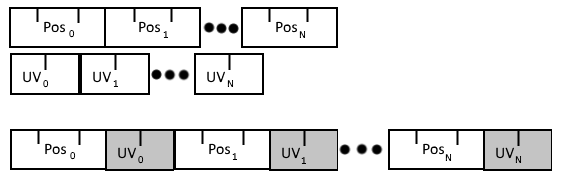
\includegraphics[width=\textwidth]{Main/Images/VertexInputLayoutVariants}
        %   \centering
        %   \caption{Layout of vertex input data when stored separately in multiple buffers (top) and interleaved in a single buffer (bottom).}
        %   \label{fig:VertexInputLayoutVariants}
        % \end{figure}

      \subsubsection{Input Assembly State}
        The input-assembly state describes how the input data to the vertex shader is interpreted.
        The most important parameter to set is the primitive topology.
        This is where the \gls{gpu} is told what kind of primitives the input data represents.
        For the purposes of this chapter, the chosen primitive topology is \lstinline{TRIANGLE_LIST}\footnote{Full name: \lstinline{VK_PRIMITIVE_TOPOLOGY_TRIANGLE_LIST}}.

        \lstinputlisting[
          label=lst:InputAssemblyStateSetup,
          caption={Input assembly state setup for chapter~\ref{cha:RenderPipeline}.},
          style=MyCppFloat,
          firstline=34,
          lastline=35,
          float
        ]
        {Main/Listings/GraphicsPipelineSetup.cpp}

      \subsubsection{Tessellation State}
        \todo[inline]{Just omit this state and subsubsection? It's nullptr in the graphics pipeline.}
        This state is only useful for the tessellation shader stage.
        In this chapter, only the vertex and fragment shader stages are in use so this state is ignored.

      \subsubsection{Viewport State}
        \label{sss:ViewportState}
        The viewport state specifies how many viewports and scissors are active in a pipeline.
        Both the viewport and scissor define a non-rotated rectangular region within the framebuffer that will be written to by shaders.
        Rendering results that would usually write to the entire extent of the framebuffer will be scaled down and displaced to fit into the viewport and cropped to be inside the scissor.
        See figure~\ref{fig:ViewportScissorSample} for an illustration of this.
        In this chapter, only one of each is used that \todo{encompass?}include the entire framebuffer.

        \begin{figure}
          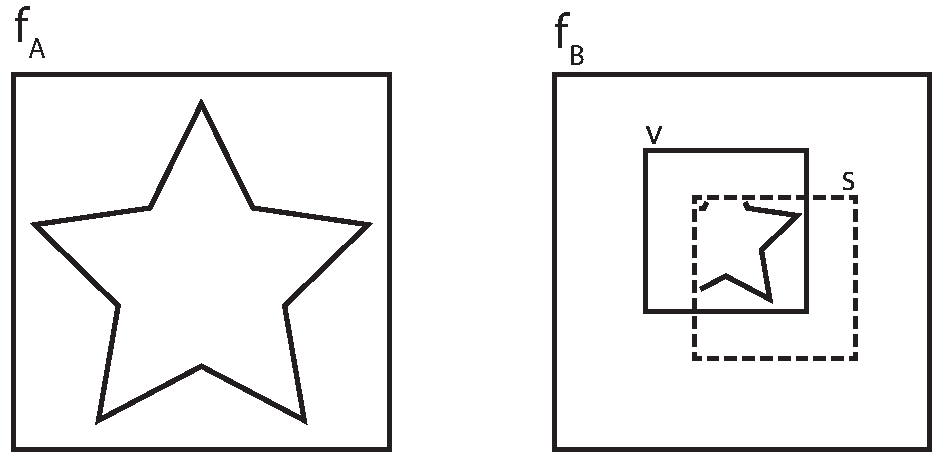
\includegraphics[width=0.666\textwidth]{Main/Images/ViewportScissorSample}
          \centering
          \caption{Framebuffer {\large$f_A$} has a viewport and scissor that contain the entire framebuffer. No transformation or cropping is performed. Framebuffer {\large$f_B$} has a viewport {\large$v$} that causes the contents to be displaced and scaled down as well as a scissor {\large$s$} that causes the remaining contents to be cropped.}
          \label{fig:ViewportScissorSample}
        \end{figure}

        There are two ways to specify the actual viewport and scissor data.\todo{Explain briefly what viewport and scissors actually do.}{}
        The simplest way is to specify it at this point directly, \todo{Try reducing the use of i.e.}i.e. when creating the graphics pipeline.

        However, this also means that the viewport and scissor data may never change during the lifetime of the pipeline.
        Changing the viewport and scissor data is necessary when the dimension of the render targets change.
        For example, when the application window is resized, the swapchain along with all swapchain images typically need to be re-created with dimensions matching the new window size, thus the viewport and scissor need to be updated as well.

        \lstinputlisting[
          label=lst:DynamicStateSetup,
          caption={Dynamic state setup for viewport and scissor state in chapter~\ref{cha:RenderPipeline}.},
          style=MyCppFloat,
          firstline=40,
          lastline=46,
          float
        ]
        {Main/Listings/GraphicsPipelineSetup.cpp}

        \lstinputlisting[
          label=lst:ViewportStateSetup,
          caption={Viewport state setup for chapter~\ref{cha:RenderPipeline}.},
          style=MyCppFloat,
          firstline=48,
          lastline=50,
          float
        ]
        {Main/Listings/GraphicsPipelineSetup.cpp}

        In order to prevent re-creating the entire graphics pipeline every time, which is a costly operation, the pipeline can be configured to accept \textit{dynamic state} as shown in listing~\ref{lst:DynamicStateSetup}.
        Dynamic state has to be set everytime when a render pass is being processed.
        Dynamic state data is recorded in command buffers and submitted along with the relevant render pass commands.

        Because dynamic state for the viewport and scissor data is used in this chapter, specifying the number of viewports and scissors as shown in listing~\ref{lst:ViewportStateSetup} is sufficient for the purpose of setting up a graphics pipeline.

      \subsubsection{Rasterization State}
        The rasterization state is used to configure the behavior of the rasterizer.
        It can be configured to control how fragments are produced and the circumstances in which they may be discarded.

        It is also used to control how primitves are rasterized.
        For example, given a triangle primitve, there are three ways for the rasterizer to produce fragments: Densely fill the entire rectangle, only produce fragments for the outline of the triangle, or just produce a fragment for each of the vertices, respectively.

        The rasterizer can also be configured to perform face culling, i.e. discarding fragments that are facing in a certain direction.
        Without this option, fragments are produced regardless of the direction they are facing.
        However, it is common to enable back-face culling, i.e. discarding fragments that would be viewed from ``behind'', for triangle meshes that form a closed object.

        In order to perform culling, the rasterizer needs to know the facing direction of a triangle.
        This facing direction is also configurable in the rasterizer state.
        It is defined by the winding order of the vertices, which is considered to be either \textit{clockwise} or \textit{counter-clockwise}.

        \lstinputlisting[
          label=lst:RasterizationStateSetup,
          caption={Rasterization state setup for chapter~\ref{cha:RenderPipeline}.},
          style=MyCppFloat,
          firstline=55,
          lastline=57,
          float
        ]
        {Main/Listings/GraphicsPipelineSetup.cpp}

        % \todo[inline]{I don't show a listing for any of the other pipeline states. This is an experiment to see how it would be if I backed the text with corresponding listings.}

        In listing~\ref{lst:RasterizationStateSetup}, the rasterizer is configured to produce densely filled polygons and does not perform any culling operations on the fragments.

      \subsubsection{Multisample State}
        \label{sss:MultisampleState}
        Multisampling is used to perform anti-aliasing, achieving a smoother appearance of jagged edges, and can be configured in the Multisample state.
        Disabling multisampling is not simply a matter of specifying the default value for all options.
        This state controls how many times the fragment shader is invoked and if a value of zero is passed as the number of samples, the fragment shader will never be invoked.

        Multisampling is not being used in this chapter so the number of samples is set to one.

        \lstinputlisting[
          label=lst:MultisampleStateSetup,
          caption={Multisample state setup for chapter~\ref{cha:RenderPipeline}.},
          style=MyCppFloat,
          firstline=62,
          lastline=63,
          float
        ]
        {Main/Listings/GraphicsPipelineSetup.cpp}

      \subsubsection{Depth Stencil State}
        Depth and stencil tests are controlled in this state.
        Individual control is provided to enable depth testing, depth writing, depth bounds testing, as well as stencil testing.
        Depth bounds and comparison operations as well as stencil operations can be configured in this state.
        The comparison operation during depth tests can also be controlled.

        In this chapter, stencil tests are disabled.
        Depth testing, on the other hand, is enabled with depth bounds of $[0, 1]$ and with the typical less-or-equal comparison operation.

        \lstinputlisting[
          label=lst:DepthStencilStateSetup,
          caption={Depth and stencil state setup for chapter~\ref{cha:RenderPipeline}.},
          style=MyCppFloat,
          firstline=68,
          lastline=72,
          float
        ]
        {Main/Listings/GraphicsPipelineSetup.cpp}

      \subsubsection{Color Blend State}
        The color blend state controls how color values produced by the fragment shader are combined, or blended, with the color that is already in the framebuffer.
        \todo{Mention `logicOp' and `blendConstants'?}
        The blend operations need to be specified for each render target individually.\todo{Mention that a pipeline is needed for each material.}{}
        Blend operations may also be turned off which simply replaces whatever was in the framebuffer with the output of the fragment shader.

        In addition to controlling blending, a color mask can be set that controls which components of the resulting color values are written to the framebuffer.
        If a color mask of 0 is supplied, the framebuffer contents will remain unchanged.
        Likewise, a color mask with all bits set to 1 will copy all color components to the framebuffer.
        It is crucial to set this value correctly, otherwise undesired behavior may be observed.

        \lstinputlisting[
          label=lst:ColorBlendStateSetup,
          caption={Color blend state setup for chapter~\ref{cha:RenderPipeline}.},
          style=MyCppFloat,
          firstline=77,
          lastline=83,
          float
        ]
        {Main/Listings/GraphicsPipelineSetup.cpp}

        In this chapter, blending is turned off and a color mask is chosen so all color components are copied to the framebuffer.

        \todo[inline]{Give an example (transparent vs. non-transparent) if there is enough time.}

      \subsubsection{Render Pass}
        \label{sss:RenderPassSetup}
        Each graphics pipeline has exactly one render pass in Vulkan.
        A render pass consists of multiple subpasses and stores information about the flow of data between subpasses and the execution of rendering commands.
        It stores framebuffer attachment and information about layout transitions at the beginning and the end of the render pass as well as between subpasses.
        Framebuffer attachments are images such as a swapchain image or a depth-buffer.
        Each of these subpasses may reference the aforementioned framebuffer attachments of the render pass.
        Dependencies of each subpass are also stored in the render pass.
        Rendering commands are always recorded to one of the subpasses of a render pass \textit{instance}.
        Command buffer recording is discussed in section~\ref{sec:BuildCommandBuffers}.

        \todo[inline]{Give an example about subpasses (post-processing) if there is enough time.}

        \lstinputlisting[
          label=lst:RenderPassAttachmentsSetup,
          caption={Setup of the attachments for the render pass used in chapter~\ref{cha:RenderPipeline}.},
          style=MyCppFloat,
          firstline=88,
          lastline=101,
          float
        ]
        {Main/Listings/GraphicsPipelineSetup.cpp}

        In listing~\ref{lst:RenderPassAttachmentsSetup}, the attachments for the render pass are being set up.
        The first attachment, attachment 0, is the render target which is actually a swapchain image.
        The format of that attachment is set to the same format as the surface.
        Like before in section~\ref{sss:MultisampleState}, the sampling count is set to 1, i.e. multisampling is not used.
        On line~4, the render pass is configured to clear the contents of the first attachment at load-time.
        The value to clear the contents with is defined in the render pass instance.
        Once the render pass has finished executing, the \lstinline{storeOp} determines what happens to this attachment.
        In this case, on line~5, the framebuffer contents are preserved.
        Alternatively, the render pass can be configured to discard the results instead but that is not the desired behavior in this particular case.

        The subsequent settings are used to control the image layout at the beginning and the end of a render pass, respectively.
        On line~6, the initial layout of the attachment is specified to be undefined.
        This tells the \gls{driver} that it may discard the contents if it sees fit.
        The previous contents of the attachment are not relevant for this render pass because the attachment is cleared as the first operation when loaded by this render pass.
        On line~7, the render pass is configured to ensure that the image layout state of the attachment is \lstinline{PRESENT_SRC}\footnote{Full name: \lstinline{VK_IMAGE_LAYOUT_PRESENT_SRC_KHR}}.
        This way no further transformations to the undrelying swapchain image have to be performed before it can be presented.

        On lines 9--14, the depth buffer attachment is configured.
        The format of this attachment is set to the format of the actual depth buffer.
        Similarly to the first attachment, the depth buffer is cleared at the beginning of the render pass.
        The \lstinline{storeOp} is set to \lstinline{DONT_CARE}\footnote{Full name: \lstinline{VK_ATTACHMENT_STORE_OP_DONT_CARE}} because the depth buffer is not used outside the render pass.
        This is also the reason why both the inital and the final layout are simply set to \lstinline{DEPTH_STENCIL_ATTACHMENT}\footnote{Full name: \lstinline{VK_IMAGE_LAYOUT_DEPTH_STENCIL_ATTACHMENT_OPTIMAL}}.

        \lstinputlisting[
          label=lst:RenderPassSubpassSetup,
          caption={Setup of the single subpass for use in chapter~\ref{cha:RenderPipeline}.},
          style=MyCppFloat,
          firstline=103,
          lastline=115,
          float
        ]
        {Main/Listings/GraphicsPipelineSetup.cpp}

        As mentioned before, a render pass consists of multiple subpasses.
        Every render pass needs at least one subpass.
        For the purposes of this chapter, a single subpass is sufficient.
        This subpass is configured as shown in listing~\ref{lst:RenderPassSubpassSetup}.

        A subpass accepts configurations for the layout of individual attachments.
        Subpasses have references to the attachments of the render pass itself.
        These attachment references contain additional information, the most important one being the layout in that subpass.
        On line~2 of listing~\ref{lst:RenderPassSubpassSetup}, the index of the referenced attachment in the render pass is set.
        On line~3, the attachment reference is configured to ensure the correct image layout for the referenced attachment during the execution of that subpass.
        Every subpass within a render pass may define their own requirements for the layout of every individual attachment.
        Image layout transitions are performed by the \gls{driver} between subpasses as needed to ensure each subpass uses the attachment in the required layout.
        The depth-stencil reference on lines 6 and 7 is referencing the remaining attachment of the render pass and requires the \lstinline{DEPTH_STENCIL_ATTACHMENT} layout for this attachment.

        Note that the depth-stencil attachment reference on line~13 is only a single element, not an array.
        Color references on line~11 and 12, on the other hand, are not limited to a single instance.
        This means that a subpass may reference many color attachments but only a single depth-stencil attachment.

        \lstinputlisting[
          label=lst:RenderPassCreation,
          caption={Creation of a render pass object using the data defined in listings~\ref{lst:RenderPassAttachmentsSetup}~and~\ref{lst:RenderPassSubpassSetup}.},
          style=MyCppFloat,
          firstline=117,
          lastline=124,
          float,
          emph={RenderPass}
        ]
        {Main/Listings/GraphicsPipelineSetup.cpp}

        And finally, the attachment and subpass information defined previously are combined and passed to the appropriate Vulkan command on line~8 in listing~\ref{lst:RenderPassCreation} to create the actual render pass object.

      \subsection{Creating Framebuffers}
      \label{subsec:CreatingFramebuffers}
        A framebuffer defines the actual attachments that will be written to during a render pass.
        For the purposes of this chapter, each framebuffer references a swapchain image and a depth buffer image.
        Because there is usually more than one swapchain image, more than one framebuffer is required.
        Otherwise the framebuffer would need to be recreated every time a new swapchain image was acquired.
        A framebuffer also has dimensions that are defined when creating that framebuffer as shown below.
        These dimensions usually correspond to the dimensions of the referenced swapchain image.

        \lstinputlisting[
          label=lst:CreatingFramebuffers,
          caption={Creation of a set of framebuffers, one for each swapchain image.},
          style=MyCppFloat,
          float,
          emph={Framebuffers}
        ]
        {Main/Listings/CreatingFramebuffers.cpp}

        The process of creating the required framebuffers is shown in listing~\ref{lst:CreatingFramebuffers}.
        At first, a plain array of framebuffer handles is allocated using host memory.
        This array contains as many elements as there are swapchain images.
        Line~2 is the beginning of a loop that produces an index for every swapchain image with each iteration.
        On lines~4--6 the attachments of the framebuffer are defined.
        The first attachment is an image view to the swapchain image with the given index.
        The second attachment is the depth buffer that is the same for each framebuffer.
        It should be noted that the attachments are image \textit{views}, not plain images.
        Images are typically never used directly in Vulkan but rather referenced via image views that control which portion of the underlying image is used and how it is accessed.
        The image views used in this chapter all encompass the entirety of the images they reference.

        Following the attachment setup, the actual framebuffer info is constructed starting on line~8.
        It contains the attachments that were just specified, the render pass this framebuffer will be used for, the dimensions of the framebuffer in terms of a width, height, and layer count.
        Specifying the render pass at this point is not a hard restriction, it defines the types of render passes this framebuffer will be compatible with.
        And finally on line~15, a framebuffer is created and stored in the array created before.

      \subsection{Creating Scene Objects}
        \label{sss:CreatingSceneObjects}
        \todo[inline]{Mention push constants?}

        When creating scene objects, there are certain facilities that need to be set up on a per-object basis.
        In the example used throughout this chapter, every object needs to know how it can be translated from an application-specific space to clip space.
        Using this information, objects may be placed in different locations in the scene.
        The shader used for rendering them reflects this and is shown in section~\ref{sss:GraphicsPipelineShaderStages}.
        The descriptor set layout of the vertex shader, explained in section~\ref{sss:GraphicsPipelineLayout}, consists of only a single uniform buffer that contains information specific to an individual scene object.
        If a single instance of this information was shared among all scene object, they would appear in the same location at once.
        Thus, a descriptor set, which adheres to the aforementioned descriptor set \textit{layout}, has to be created for each rendered object in the scene.

        The listings presented in this section are specific to each scene object.
        These listings may be thought of as depicting code inside of a loop that iterates all objects.

        \lstinputlisting[
          label=lst:AllocateUniformBuffer,
          caption={Allocation of a buffer object that will only be used as uniform buffer. Details about memory allocation are omitted.},
          style=MyCppFloat,
          firstline=1,
          lastline=9,
          float,
          emph={UniformBufferMemory, UniformBuffer}
        ]
        {Main/Listings/CreateSceneObjects.cpp}

        The first action to perform is to allocate a buffer for each object.
        This is shown in listing~\ref{lst:AllocateUniformBuffer}.
        When creating a buffer, Vulkan needs to know what the buffer will be used for.
        In this case the buffer will only be used as a uniform buffer object as specified on line~2.
        Details of allocating the memory for this buffer are omitted.
        However, for the purposes of this chapter, it is required that the memory is host-visible.
        Host-visible memory is needed in order to update the data without involving a separate command buffer that would upload and copy data on the device to the target buffer.
        This is important in the render loop discussed in section~\ref{sec:RenderLoop}.
        In order to make this buffer available during rendering, it needs to be bound to proper facilities that because buffer objects do not provide information about where or how they are used in a shader.
        This information is provided by descriptor sets.
        Every descriptor set is tied to a one or more descriptor set layouts.
        Only a single layout is used in this case which has been defined in section~\ref{sss:GraphicsPipelineLayout}.
        Descriptor sets can be bound to a command buffer to be used for a specific graphics pipeline, which is shown later when rendering commands are recorded in section~\ref{sec:BuildCommandBuffers}.

        \lstinputlisting[
          label=lst:DescriptorPoolCreation,
          caption={Creation of a descriptor pool which only supports allocating a single uniform buffer descriptor.},
          style=MyCppFloat,
          firstline=11,
          lastline=19,
          float,
          emph={DescriptorPool}
        ]
        {Main/Listings/CreateSceneObjects.cpp}

        \lstinputlisting[
          label=lst:DescriptorSetAllocation,
          caption={Allocation of a descriptor set.},
          style=MyCppFloat,
          firstline=21,
          lastline=26,
          float,
          emph={DescriptorSet}
        ]
        {Main/Listings/CreateSceneObjects.cpp}

        Descriptor sets are allocated from descriptor pools which also manage the underlying memory used by descriptor sets.
        The relationship between a descriptor pool and descriptor sets is similar to command pools and command buffers.
        Compared to command pools, however, descriptor pools are limited to a certain number of descriptor types that can be allocated from it.
        These limits are defined by the application when a descriptor pool is created as shown in listing~\ref{lst:DescriptorPoolCreation}.
        On lines~2~and~3, the limit for uniform buffer descriptors is set to allow only a single allocation of that type.
        This limitation information is then used on line~8 to create the descriptor pool on line~9.
        The allocation of the descriptor set is shown in listing~\ref{lst:DescriptorSetAllocation}.
        Tying the descriptor set to a descriptor set layout is shown on line~4.


  \section{Command Buffer Recording}
  \label{sec:BuildCommandBuffers}
    Rendering in Vulkan is done by issuing rendering commands.
    These commands are not dispatched to the \gls{gpu} directly but recorded into a \textit{command buffer} which is submitted to a device queue for execution.
    Submitted commands may be executed out-of-order, i.e. in a different order than they were recorded, if rearranging commands does not affect the resulting data.
    The \gls{driver} may do this in order to improve performance.
    This is analogous to how a compiler may rearrange instructions when performing optimizations to the code if this operation produces compatible results.
    Command buffers have been introduced in chapter~\ref{cha:VulkanOverview}, specifically section~\ref{sec:CommandBuffers}.

    \lstinputlisting[
      label=lst:CreateCommandBuffer,
      caption={Creation of a command pool and allocation of a command buffer.},
      style=MyCppFloat,
      firstline=1,
      lastline=9,
      float
    ]
    {Main/Listings/CreateCommandBuffer.cpp}

    Command buffer objects are created using \textit{command pools} as shown in listing~\ref{lst:CreateCommandBuffer}.
    Command pools manage the memory of the command buffers created from them.
    A command buffer is either in the \textit{initial}, \textit{recording}, or \textit{executable} state.
    The contents of a command buffer are immutable for as long as that command buffer is \textit{executable}.
    Resetting a command buffer clears its contents and reverts it to the \textit{initial} state.
    It must be noted that submitting a command buffer also does not clear its contents.
    This means that command buffers may be recorded once and executed multiple times.
    This can be very useful when recording a series of render commands for state .
    It also improves performance insofar that the \gls{driver} is able to keep frequently used command buffers in \gls{gpu} memory, reducing required communication overhead between the \gls{cpu} and the \gls{gpu} and thus, reducing required bandwidth for data transmission.
    An example for such kinds of command buffers is for rendering state scene geometry.
    This kind of geometry is does not change with time, hence the commands required for rendering also do not change.

    For the purposes of this chapter, command buffers will only be recorded once and submitted in the render loop in section~\ref{sec:RenderLoop}.
    The framework defined before allows this to be possible because all objects in the scene are static in terms of rendering commands.
    However, this is only true because per-object shader data is stored in uniform buffer objects as established in section~\ref{sss:CreatingSceneObjects}.
    Uniform buffers are independent of the rendering commands and can be updated directly using memory mapping operations.
    Alternatively to uniform buffers, \textit{push constants} may be used to supply data to be used in shaders.
    Compared to uniform buffer objects, push constants have certain limitations that need to be considered.

    For each shader module, only a single \textit{push constant block} may be declared.
    The size of such a block is limited.
    The Vulkan specification requires that \glspl{driver} support sizes of at least 128 bytes but larger blocks may also be supported.
    The upper limit is specific to individual devices and can be queried using the Vulkan \gls{api}.
    Sizes of 256 bytes are common on current \gls{nvidia} hardware.
    Because of small sizes like this, push constants are likely to be stored in registers directly as opposed to uniform buffers which are stored in \gls{vram}.
    A note in section~13.2.6 also hints that using push constants may yield improved performance in terms of execution speed.

    The way values are supplied for push constant blocks is different from how a uniform buffer object is updated.
    Push constant values are updated using commands and are recorded to command buffers.
    This means that these values may be different for each recorded command buffer.
    If values are stored in the push constant block that change every frame, such as the model-view-projection matrix of a scene object, command buffers need to be recorded every frame.

    \todo[inline]{Put a subsection here?}
    % \subsection{Rendering a Scene Object}
      % In this section, the necessary steps to record rendering commands for all scene objects are shown and explained.

      \lstinputlisting[
        label=lst:BeginCommandBuffer,
        caption={Start of the recording of a command buffer.},
        style=MyCppFloat,
        firstline=1,
        lastline=2,
        float
      ]
      {Main/Listings/CommandBufferRecording.cpp}

      % The first action that has to be performed is to start command buffer recording.
      Before issuing rendering commands, the command buffer has to be put into \textit{recording} state, which can be seen on line~2 of listing~\ref{lst:BeginCommandBuffer}.
      When beginning a command buffer, additional information can be passed in the \lstinline{VkCommandBufferBeginInfo} structure which can be seen on line~1.
      For example, this can be used to inform Vulkan that this particular command buffer is only submitted once which might allow the \gls{driver} to perform optimizations.
      For the purposes of this example, the default values are sufficient.

      \lstinputlisting[
        label=lst:DynamicStateUpdate,
        caption={Updating dynamic render pass state using Vulkan commands.},
        style=MyCppFloat,
        firstline=4,
        lastline=13,
        float,
        emph={vkCmdSetViewport, vkCmdSetScissor}
      ]
      {Main/Listings/CommandBufferRecording.cpp}

      Once the command buffer is \textit{recording}, the dynamic state can be set.
      As defined in section~\ref{sss:ViewportState} and shown in listing~\ref{lst:DynamicStateSetup}, the dynamic state to update include the viewport and scissor.
      \todo{Highlight vkCmdSet* in the listings?}
      The commands for updating this state are shown in listing~\ref{lst:DynamicStateUpdate}.
      The viewport is set to include the entire framebuffer on lines~2--3 as well as the entire depth buffer extent on lines~4--5.
      The scissor is set to contain the entire viewport on line~9, effectively disabling cropping of the resulting image.

      Dynamic state values are part of the command buffer.
      These values are read by graphics pipelines when executing draw commands without clearing them.
      This means that dynamic state only has to be set once for every command buffer if the values never change which why dynamic state updates are the first commands recorded in the example of this chapter.
      These commands may be recorded at a later point if need be, but no later than before the first draw command is recorded.
      Additionally, setting these values is only necessary if the graphics pipeline has been set up to accept viewport and scissor data as dynamic state.
      Graphics pipelines that are not instructed to look for dynamic state will simply ignore the data in the command buffer and instead use the data supplied at pipeline creation.

      \lstinputlisting[
        label=lst:BeginRenderPass,
        caption={Creation of a render pass instance within a command buffer.},
        style=MyCppFloat,
        firstline=15,
        lastline=25,
        float,
        emph={vkCmdBeginRenderPass}
      ]
      {Main/Listings/CommandBufferRecording.cpp}

      In the next step, a render pass is started which results in the creation of a \textit{render pass instance}.
      This render pass instance is associated with a specific framebuffer on line~7 and clear values on line~10~and~11 that are used to clear attachment contents if their \lstinline{loadOp} is set to \lstinline{CLEAR}\footnote{Full name: \lstinline{VK_ATTACHMENT_LOAD_OP_CLEAR}}.
      The \lstinline{loadOp} settings were specified for each attachment in section~\ref{sss:RenderPassSetup}.
      Another property of the render pass instance is the render area on line~8.
      As can be seen, it set to the same value as the scissor that was set before.
      The render area is used to control which pixels of the framebuffer are affected in the active render pass.
      This is used to minimize necessary work for the \gls{gpu}.
      As per the Vulkan specification, a render area that is smaller than the entire framebuffer may affect performance negatively.
      A render area that is larger than the framebuffer is invalid.

      When beginning a render pass, Vulkan also needs to be told about whether secondary command buffers will be used or not.
      For the purposes of this chapter, only a single primary command buffer is used in a single subpass, which is why the render pass is instructed to inline render commands directly in the primary command buffer, disallowing execution of secondary command buffer.
      More information about command buffers was given in section~\ref{sec:CommandBuffers}.

      \todo[inline]
      {
        If the reader is not following carefully, it might seem like scissors do the same thing as the render area, which is not strictly true.
        First, there may be many scissors but only a single render area at once.
        Secondly, scissors are specified as part of the pipeline while the render area is part of the render pass \textbf{instance}.
        Should I mention and explain this?
        It should be obvious from the text and would be redundant.
      }

      \lstinputlisting[
        label=lst:ObjectRenderingLoop,
        caption={Rendering of all scene objects.},
        style=MyCppFloat,
        firstline=27,
        lastline=40,
        float
      ]
      {Main/Listings/CommandBufferRecording.cpp}

      Now that a render pass instance is set up, draw commands can be recorded.
      Because there are multiple objects in the scene that need to be rendered, this will happen in a loop as can be seen on line~1 in listing~\ref{lst:ObjectRenderingLoop}.
      The first command causes the binding of a descriptor set with a specific pipeline layout.\todo{Reference where descriptor sets and pipeline layouts are first explained.}{}
      \todo{Explain the other, optional arguments?}

      \todo[inline]{Explain why the pipeline is bound later than the render pass. Maybe mention that a render pass may be shared between multiple pipelines.}
      Afterwards, the command to bind the graphics pipeline is recorded on line~9.
      It is explicitly stated that the passed pipeline object is a graphics pipeline.

      \todo{Too informal?}With a pipeline in place, the vertex buffer and index buffer objects are bound.
      In both cases, the entire buffers are used, which is why all offsets are set to zero.
      As can be seen on line~11, multiple vertex buffers can be bound at once.
      Vertex buffers may be bound to different binding locations using the second argument to the depicted Vulkan API call, as long as these locations are valid for the given pipeline layout.
      In the case of this example, only a single vertex buffer is used per object that is bound to location 0.
      The indices in the index buffer contains unsigned 32~bit integer values.
      This information is passed to Vulkan on line~12.

      Following all the binding commands, the actual drawing command is issued.
      There are several drawing commands available but for the combination of objects that are bound only indexed drawing is valid.
      Because rendering is supposed to be done by using the bound index buffer, the drawing command to be recorded is \lstinline{vkCmdDrawIndexed}.
      The arguments are, in order, the number of indices to read from the index buffer, the number of instances to render, the index of the index buffer to use, an offset that is added to each value in the index buffer before it is used to perform vertex lookups, and finally the ID of the first instance to draw.
      Because instanced rendering is not intended, the instance count is set to 1 and the ID of the first instance is set to 0.
      The index buffer is assumed to be set up to reference every vertex directly.
      This means that the entire index buffer can be used with both offsets set to 0 and the count set to the number of available indices in the index buffer.

      \lstinputlisting[
        label=lst:ConcludingCommandBufferRecording,
        caption={Completion of the render pass and command buffer recording.},
        style=MyCppFloat,
        firstline=42,
        lastline=43,
        float
      ]
      {Main/Listings/CommandBufferRecording.cpp}

      Once all commands have been recorded, the render pass and the command buffer may be ended.
      This is shown in listing~\ref{lst:ConcludingCommandBufferRecording}.
      This transitions the command buffer from \textit{recording} to \textit{executable} state.
      The function \lstinline{vkEndCommandBuffer}, as seen on line~2, returns a status code of type \lstinline{VkResult}.
      If an error occurred during command buffer recording, all subsequent \lstinline{vkCmd*} calls will be ignored and an error code will be return when the command buffer is ended.
      For example, the command buffer may run out of memory early on and signal this once recording has ended.

      The command buffer is now ready for submission to a queue and execution on the \gls{gpu}.
      This is covered in section~\ref{sec:RenderLoop}.\todo{More verbose conclusion paragraph? Or remove it?}{}

      In the process presented above, only a single command buffer was recorded.
      For small amounts of commands like in this case, it might be beneficial to allocate a command buffer for each framebuffer and perform the recording for each of them.
      This avoids re-recording of command buffers every time a new swapchain image is acquired.


  \section{Rendering Loop}
  \label{sec:RenderLoop}
    \todo[inline]{Rather simple because of pre-recording command buffers.}
    \todo[inline]{Update shader data (UBOs, dynamic state, etc).}
    \todo[inline]{Possibly explain push constants.}
    \todo[inline]{Acquire swapchain image.}
    \todo[inline]{Submit command buffers.}
    \todo[inline]{Present swapchain image.}
    \todo[inline]{Sync for submission and presenting (render semaphore, present semaphore) so swapchain image isn't used for rendering while presenting and vice versa. Also image layout transition happens with commands, meaning sync is necessary!}
    \tbd

    \lstinputlisting[
      label=lst:RenderLoop_SemaphoreCreation,
      caption={Creation of two semaphores used in the render loop.},
      style=MyCppFloat,
      firstline=1,
      lastline=5,
      float
    ]
    {Main/Listings/RenderLoop.cpp}

    \lstinputlisting[
      label=lst:RenderLoop_ShaderDataUpload,
      caption={Creation of two semaphores used in the render loop.},
      style=MyCppFloat,
      firstline=7,
      lastline=22,
      float
    ]
    {Main/Listings/RenderLoop.cpp}

    After the camera has been updated, the uniform buffers of each object in the scene have to be updated as well.
    Listing~\ref{lst:RenderLoop_ShaderDataUpload} shows the loop in which this is done.
    For each object, the model-view-projection (MVP) is computed.
    Afterwards, the buffer memory is mapped to an actual memory location in \gls{cpu} accessible \gls{ram}.
    The computed MVP matrix is then copied to the mapped memory region on line~12.
    On line~13, the memory mapping is undone to allow the \gls{driver} to reuse the memory region.

    \lstinputlisting[
      label=lst:RenderLoop_AcquireNextImage,
      caption={Creation of two semaphores used in the render loop.},
      style=MyCppFloat,
      firstline=21,
      lastline=29,
      float
    ]
    {Main/Listings/RenderLoop.cpp}

    The following step is to acquire the next free image from the presentation engine to be used for rendering.
    The necessary function call is shown in listing~\ref{lst:RenderLoop_AcquireNextImage}.
    Because this function may potentially block for as long as no swapchain image is available, it accepts a timeout argument.
    In this case, the maximum value for an unsigned 32~bit integer is passed, effectively waiting as long as possible for the function to return.
    This function also accepts a semaphore as fourth argument.
    This semaphore is needed because the presentation engine might not be finished reading from the image yet.
    Once the presentation engine is done processing the image, the semaphore is signaled.

    \lstinputlisting[
      label=lst:RenderLoop_QueueSubmission,
      caption={Submission of a command buffer to the device queue for rendering. Several semaphore are installed to ensure proper synchronization between the host and the device.},
      style=MyCppFloat,
      firstline=32,
      lastline=45,
      float
    ]
    {Main/Listings/RenderLoop.cpp}

    The next task depends on the exact setup of the system.
    If command buffers were created, one for each framebuffer, then the one corresponding to the acquired image may directly be submitted.
    This is assumed in listing~\ref{lst:RenderLoop_QueueSubmission}.
    If, on the other hand, only a single command buffer was allocated, it needs to be re-recorded at this point.
    Ideally, the application has put everything that is described in section~\ref{sec:BuildCommandBuffers} into a function which could now be called.
    However, this means that the \gls{driver} has to evaluate and upload the command buffer all over again.
    That is why pre-recording command buffers per framebuffer might be beneficial.
    The best course of action may vary and is a matter of performance evaluations on a per-application and possibly even per-platform basis.

    The command buffer that is in \textit{executable} state is now submitted to the queue for execution in listing~\ref{lst:RenderLoop_QueueSubmission}.
    When submitted command buffers, a number of semaphores may be passed that are used to ensure proper synchronization between the device and the host.
    On line~7, the semaphore that was used when the current swapchain image was acquired is used.
    This semaphore will be waited on in the stages specified on line~5.
    In this particular case it is set up so that color attachment writes are only performed after the presentation engine no longer reads from the image, thus properly synchronizing read and write access to the image.
    The semaphore on line~9 will be signaled once submitted command buffers have finished execution.
    This semaphore is used when presenting the image, which is explained next.


    \todo[inline]{Next action is command buffer submission. Mention that it must be re-recorded here is push constants would be used.}

    \lstinputlisting[
      label=lst:RenderLoop_QueuePresent,
      caption={Creation of two semaphores used in the render loop.},
      style=MyCppFloat,
      firstline=47,
      lastline=57,
      float
    ]
    {Main/Listings/RenderLoop.cpp}

    Once command buffers have been submitted, the image they produce is presented to the application window.
    This process is shown in listing~\ref{lst:RenderLoop_QueuePresent}.
    First, the swapchain to perform the presentation with is specified on line~5.
    On line~6, the index of the image to present is given.
    Afterwards, on line~8, a semaphore is supplied.
    This semaphore will be waited on by the presentation engine before performing any reads on the specified image.
    It is the same semaphore shown earlier that is signaled once the submitted command buffers finished execution.
    In other words, the presentation engine waits until the \gls{gpu} has finished writing to the image before reading from the image in order to present it.
    On line~9, the actual present call is performed.

    % \lstinputlisting[
    %   label=lst:RenderLoop_QueueWaitIdle,
    %   caption={Creation of two semaphores used in the render loop.},
    %   style=MyCppFloat,
    %   firstline=59,
    %   lastline=63,
    %   float
    % ]
    % {Main/Listings/RenderLoop.cpp}



  % \section{Window Resizing}
  %   \todo[inline]{Should I actually add this section? (Only if there's enough time.)}
  %   \tbd

  \section{Multi-threaded Rendering}
  \label{sec:MultithreadedRendering}
    \todo[inline]{Introduction to this chapter. Motivation. Additional complexity. Applications must be sure they gain anything from using multi-threading.}
    As mentioned in chapter~\ref{cha:VulkanOverview}, Vulkan API calls are not synchronized implicitly by the \gls{driver} in order to facilitate multi-threaded processing.
    However, this does not mean that multi-threading on the \gls{cpu} has not been taken into account when Vulkan was designed.
    There are actually several ways of utilizing multiple threads for rendering with Vulkan.
    Creating resources and recording command buffers from multiple threads are explored in the following subsections.

    \subsection{Multi-threaded Command Buffer Recording}
      A naive approach to utilize multi-threading is to create several command buffers and assign them to multiple threads.
      These threads would then record commands to their assigned command buffers and submit them to a device queue.
      Unfortunately, there are some problems with this approach.
      According to sections~5.3~and~5.4 of the Vulkan specification\cite{vkspec}, the host application is responsible for synchronizing interactions with command buffers and submitting them to device queues.

      % Problem with command buffers and multi-threaded access.
      Command buffer access is not thread-safe.
      This is because memory used by command buffers is managed by the parent command pool.
      The actual algorithms used for managing memory are left to the \gls{driver}.
      % Done for implementations to be more memory efficient.
      This allows command pools efficient handling of memory operations performed by multiple command buffers, e.g. by allocating more memory than is currently needed and reassigning it as more is requested.
      % Command buffers work on memory managed by parent command pool.
      Because command pools are free to manage memory as they see fit, any operation on a command buffer may trigger side-effects that affect other command buffers created from the same pool.
      This fact alone makes command buffers unsuitable to be shared across multiple threads without synchronization.

      % Command pools do not depend on anything else.
      Command pools, on the other hand, are independent objects.
      The memory they manage is only used for command buffers they created.
      Whenever available memory is no longer sufficient, new memory from the host is requested, optionally using a application-supplied allocator.
      This allocator needs to synchronize low-level allocations, like the C standard library function \lstinline{malloc} already does.
      % Thus solution is to assign each thread its own command pool.
      Synchronization of low-level memory allocation is certainly not as costly as synchronizing each command buffer access.
      Typically, those low-level memory allocations do not happen very often.
      It is likely that command pool implementations strive for minimal host allocations.

      Command pools effectively do not need to be manually synchronized across multiple threads if they are not shared between them.
      In addition, command buffers created from such command pools inherit the same properties.
      Thus, it is more suitable to assign one or more command pools per thread.
      % Threads then allocate and record into as many command buffers as needed.
      Each thread is then free to allocate and record into as many command buffers as needed without having to conduct fine-grained synchronization.

      % Let main thread submit command buffers by sharing a datastructure with synchronized access.
      In order for command buffers allocated on other threads to be submitted to the device queue, the main thread may provide a shared datastructure that is capable of containing command buffer objects.
      Access to this shared container would be synchronized using traditional synchronization methods.
      % Turns the initial problem into well-understood producer-consumer problem\cite{EWD:EWD329}.
      % Solves the inital queue submission problem.
      This effectively creates the well-understood producer-consumer scenario\cite{EWD:EWD329} and solves the initial queue submission problem.

      \todo[inline]{Prev paragraph is just a suggestion. May be better to do differently. Depends on application.}

      \subsubsection{Command Buffer Management Considerations}
        % ... There is another problem with the system mentioned above.
        % ... It is also recommended to assign more than one command pool to an individual thread.
        % ... While a command buffer is being processed, i.e. once it has been submitted but has not finished execution yet, the command buffer should not be modified.
        % ... The reason why multiple pools should be used instead of simply creating new command buffers from the same pool is because of the underlying memory model.

        % ... In the previously described scenario, each thread has exactly one command pool that is used to create multiple command buffers from.
        % ... Commands are recorded to these command buffers and are submitted in batches to the device for execution.
        % ... Vulkan specifies some restrictions on what may be done with command buffers that are pending execution.
        % ... For example, the application should not free a command buffer that is pending execution.

        % Command buffers need to be kept alive while pending execution.
        Vulkan prohibits modifying submitted command buffers that are pending execution on the device.
        This includes freeing these command buffers, i.e. the application is responsible for keeping them alive as long as they are pending execution.
        In practice, this effectively means command buffers submitted in batches may only be modified or reused once the entire submission has finished execution because it is hard to predict when individual commands are processed if more than one command buffer is submitted.
        Out-of-order execution is one reason for this unpredictability.
        The simplest way to solve this problem is to just use new command buffers for every new batch submission.
        This poses some management overhead since individual command buffers need to be associated to these batches in some way in order to be freed or reused.
        Vulkan does not do this automatically.
        Otherwise, if command buffers are never freed, the application ends up allocating a lot more than necessary, effectively leaking memory.

        % Command pools better than just using command buffers because of decoupled underlying memory and clean separation of concern.
        A better way might be to use command pools for this purpose.
        Managing command buffers is already what they do and it also offers a clean separation of concerns between the different batches of command buffers.
        In other words, using command pools to allocate command buffers that are submitted together provides a way to manage these command buffers using standard methods.
        Vulkan allows command pools to be reset, effectively resetting all command buffers spawned from them.
        This means that command pools may be reused after their associated batch of submitted command buffers has finished execution.
        When resetting a command pool, the host application is free to choose whether memory allocated by that command pool should be released or not.
        If a command pool is going to be reused, and the memory is not released, this command pool can directly start producing command buffers without causing additional allocation overhead.
        This provides a clean way for managing command buffer lifetimes without the need to use anything but the Vulkan \gls{api} itself.

        \todo{Describe what they did differently?}Similar approaches have been described by industry experts such as Marius Bjørge\cite{bjorge:multithreadingvulkan} in his blog post about multi-threading in Vulkan as well as Mathias Schott\cite{mschott:vulkan_multi_threading} in his talk entitled ``Vulkan multi-threading''.

        Care must be taken, however, in cases where the amount of memory required by a command buffer is not steady during its lifetime.
        For example, when transitioning from a large \gls{3d} scene, with many objects to render, to a small scene with less draw calls to perform, the memory requirements of each command buffer may be lowered considerably for the new scene.
        In cases like this, it might make sense to reset all relevant command buffers, freeing their associated memory.
        Switching from a small scene to larger one is not a problem, of course, because the command buffer will simply allocate enough memory for the new scene.


    \subsection{Multi-threaded Resource Creation}
      \todo[inline]{Mention staging buffers somehow?}
      Vulkan applications need to create resources such as images and shaders.
      Loading and creating these resources may take a considerable amount of time, depending on the data in question.
      Images, for example, can be quite large.
      They may also have to be transformed in some way which also consumes computation time.
      Shaders need to be compiled (by the \gls{driver}) and bound to a Vulkan pipeline.
      Many of these time consuming operations work more or less independently from the rest of the system, depending on the specific operation.
      This makes them interesting candidates for execution on multiple threads.
      However, the use of multi-threaded resource creation introduces additional complexity to the system.

      First of all, an application has to decide how many threads are actually needed for resource creation.
      It is possible that only one dedicated resource creation thread is sufficient for many applications.
      The actual number of resource creation threads depends on the application.

      All resource creation threads need device memory in one way or another.
      There are basically two ways of accomplishing this without race conditions.
      The first way is to preallocate the memory that is available for each thread.
      This method does not require synchronization between threads because each is assigned a memory region that is not overlapping memory from other threads.
      The second way is to assign a memory allocator to each thread that internally synchronizes the calls.
      This method does not require the main thread to know the size of the resources each thread creates but memory allocations need to be synchronized.
      Again, the method of choice depends on the application.

  %!TEX root = ../Main.tex

\chapter{Conclusion}
\label{cha:Conclusion}
  \todo[inline]{API quality. Explain and discuss why the API is called `modern', `highly efficient', and `explicit'.}
  \todo[inline]{Highly active development. LunarG provides more and more improved layers with each release.}
  \todo[inline]{Driver's are slow to keep up. No windows support from Intel for now.}
  \todo[inline]{Hard to learn, but probably worth it. Validation layers are awesome!}
  \todo[inline]{Mention Valve's plans for pipeline caches? Download pipeline caches when installing games.}
  \tbd



  \newpage
  \pagenumbering{Roman}


  %
  % Bibliography
  %
  \newpage
  % \nocite{*}
  \printbibliography[heading=bibintoc,title=Bibliography]


  %
  % Glossary
  %
  \printnoidxglossaries

  %
  % Appendix
  %
  %!TEX root = ../Main.tex

\appendix


%
% List of Listings
%
\renewcommand\lstlistlistingname{List of Listings}
% \addcontentsline{toc}{chapter}{\lstlistlistingname}
\lstlistoflistings


%
% List of Figures
%
\listoffigures


%
% List of Tables
%
% \listoftables


% \chapter{Prototype Source Code}
%   \label{cha:PrototypeSourceCode}
%   \todo[inline]
%   {
%     Goals:\\
%     -- Refer to the disc that came with the thesis document.\\
%     -- Also refer to GitHub. Make sure the source code is in the MastersThesis repo.\\
%   }
%   \tbd


%
% Document Source Code
%
\chapter{Document Source}
  The sources of this document can be found on GitHub using the following \gls{url}.
  Published versions of this document can also be found there in the \textit{releases} section.
  \newline

  \noindent
  \url{https://github.com/Manuzor/MastersThesis}
  \newline

  \noindent
  The published version of this document is \lstinline{v1.0} and can be found using the following \gls{url}.
  \newline

  \noindent
  \url{https://github.com/Manuzor/MastersThesis/tree/v1.0}


%
% Prototype Source Code
%
\chapter{Prototype Source Code}
  During the development of this document, another project has been developed concurrently.
  The project is written in \gls{cpp} and uses the Vulkan graphics \gls{api}.
  It was mainly used for experimenting with Vulkan and everything closely involved.
  The project is only losely connected to this document but may still provide a valuable resource to the reader.
  \newline

  \noindent
  \url{https://github.com/Manuzor/VulkanExperiments}


\end{document}
